\documentclass[11pt]{article}
% Fix font encoding (resolves OMS/cmtt font shape warnings)
\usepackage[T1]{fontenc}

% ── Geometry & Spacing ────────────────────────────────────────────────────────
\usepackage[top=1.1in, bottom=1.1in, left=1.25in, right=1.25in]{geometry}
\usepackage{setspace}
\setstretch{1.15}

% ── Core Packages ─────────────────────────────────────────────────────────────
\usepackage{lmodern}   % must come after fontenc
\usepackage{textcomp}
\usepackage{amsmath,amssymb,amsthm}
\usepackage{graphicx}
\usepackage{booktabs}
\usepackage{algorithm}
\usepackage{algpseudocode}
\usepackage{hyperref}
\usepackage{url}
\usepackage{xcolor}
\usepackage[inline]{enumitem}
\usepackage[final,babel=false]{microtype}
% Suppress residual microtype/LaTeX warnings
\usepackage{silence}
\WarningFilter{latex}{Command \showhyphens has changed}
\usepackage{multirow}
\usepackage{float}
\usepackage{pgfplots}
\pgfplotsset{compat=1.18}
\usepackage{tikz}
\usetikzlibrary{arrows.meta,positioning,shapes,fit,backgrounds,shadows}
\usepackage{listings}
\usepackage{caption}
\usepackage{subcaption}
\usepackage{parskip}

% ── Hyperref Setup ─────────────────────────────────────────────────────────────
\hypersetup{
  colorlinks=true,
  linkcolor=blue!60!black,
  citecolor=green!50!black,
  urlcolor=blue!70!black,
}

% ── Listings (Rust code) ───────────────────────────────────────────────────────
\definecolor{rustbg}{rgb}{0.97,0.97,0.97}
\definecolor{rustkw}{rgb}{0.12,0.29,0.60}
\definecolor{rustcmt}{rgb}{0.36,0.48,0.36}
\definecolor{ruststr}{rgb}{0.58,0.10,0.10}
\lstdefinelanguage{Rust}{
  keywords={pub,fn,async,await,let,mut,struct,enum,impl,for,if,else,match,use,
             mod,crate,self,return,true,false,type,where,trait,Box,Vec,Option,
             Result,Some,None,Ok,Err,String,usize,f64,u64,bool},
  keywordstyle=\color{rustkw}\bfseries,
  comment=[l]{//},
  morecomment=[s]{/*}{*/},
  commentstyle=\color{rustcmt}\itshape,
  stringstyle=\color{ruststr},
  morestring=[b]",
  sensitive=true
}
\lstset{
  language=Rust,
  backgroundcolor=\color{rustbg},
  basicstyle=\ttfamily\footnotesize,
  breaklines=true,
  frame=single,
  framerule=0.4pt,
  rulecolor=\color{gray!40},
  numbers=left,
  numberstyle=\tiny\color{gray},
  numbersep=8pt,
  tabsize=4,
  captionpos=b,
  columns=fullflexible,
}

% ── Theorem Environments ───────────────────────────────────────────────────────
\newtheorem{definition}{Definition}
\newtheorem{proposition}{Proposition}
\newtheorem{remark}{Remark}

% ── Title ──────────────────────────────────────────────────────────────────────
\title{
  \vspace{-0.5em}
  \LARGE\textbf{Hyper-Stigmergic Morphogenesis II}\\[0.4em]
  \large A Federated Multi-Agent Hypergraph System\\
  with Emergent Self-Improvement
  \vspace{-0.3em}
}

\author{
  \textbf{Arnaud Bellemare} \\[0.2em]
  Permutation Research \\
  \texttt{research@permutation.ai}
}

\date{}

% ══════════════════════════════════════════════════════════════════════════════
\begin{document}
\maketitle
\thispagestyle{empty}

% ── Abstract ──────────────────────────────────────────────────────────────────
\begin{abstract}
\noindent
We present \textbf{Hyper-Stigmergic Morphogenesis~II} (HSM-II), a novel multi-agent
system implemented in Rust that combines hypergraph-structured shared memory,
role-based evolutionary bidding, and federated knowledge propagation to achieve
emergent collective intelligence. HSM-II operationalises \emph{stigmergy}---the
indirect coordination mechanism observed in social insects~\cite{grasse1959}---at
the level of hyperedge formation and modification across a distributed network of
world-instances. The central data structure is a hypergraph whose edges carry
ontological tags, learned embeddings, and scoped visibility
(\textsc{Local}/\textsc{Shared}/\textsc{Restricted}), enabling fine-grained
knowledge governance. Ten heterogeneous agents, differentiated by four drives
(curiosity, harmony, growth, transcendence) and six roles (Architect, Catalyst,
Chronicler, Critic, Explorer, Coder), compete and cooperate via three
complementary bidding mechanisms: softmax temperature selection, Pareto
multi-objective selection, and Group Relative Policy Optimization (GRPO)
reinforcement updates~\cite{shao2024grpo}. Three emergent subsystems extend
the core: a \textbf{Council} module for structured multi-agent deliberation,
a \textbf{Dynamic Kinetic Stability (DKS)} module for self-replication dynamics,
and an \textbf{OptimizeAnything} engine for GEPA-style artifact optimization.
A four-network hybrid memory architecture fuses semantic, BM25, graph-traversal,
and temporal recall using Reciprocal Rank Fusion. Federation is achieved through
an HTTP protocol over an axum/tokio stack, with a meta-hypergraph $H^*$ governing
cross-system trust and conflict resolution. Empirical evaluation demonstrates
consistent coherence growth, skill distillation convergence, and robust federation.
\end{abstract}

\tableofcontents
\newpage

% ── 1. Introduction ────────────────────────────────────────────────────────────
\section{Introduction}
\label{sec:intro}

Collective intelligence in biological systems arises not from centralised
coordination but from local interactions mediated by a shared environment.
Ants deposit pheromone trails that other ants modify; termites build structures
whose geometry guides further construction. This principle---\emph{stigmergy}---has
inspired generations of computational models~\cite{grasse1959,dorigo1996}, yet
existing systems rarely exploit the full representational power of hypergraphs,
integrate symbolic reasoning with neural self-improvement, or federate knowledge
across distributed instances with principled trust dynamics.

The design of artificial systems capable of open-ended self-improvement poses five
fundamental challenges. A system must be able to (1)~represent structured knowledge
with sufficient expressiveness, (2)~coordinate heterogeneous agents without central
bottlenecks, (3)~evaluate and apply mutations that genuinely improve fitness,
(4)~reason symbolically about its own state, and (5)~propagate and validate
knowledge across distributed peers without catastrophic interference. HSM-II
addresses all five challenges in a unified architecture.

The system's central world---\texttt{HyperStigmergicMorphogenesis}---is a
hypergraph environment that ten typed agents continuously modify. Modification
actions are gated by a tri-modal bidding system incorporating classical softmax
selection, Pareto-optimal multi-objective selection, and GRPO-style reinforcement
updates~\cite{shao2024grpo}. A self-improvement cycle evaluates typed mutations
against a coherence-novelty objective. Symbolic reasoning via parallel Prolog
braids operates as a System~2 process, while a rolling \texttt{LivingPrompt} and
CARA reflection loop constitute System~1~\cite{latimer2025cara}. Hierarchical
skills are distilled from trajectory experience using SkillRL principles and evolved
via Bayesian confidence updates. A consensus jury pipeline validates skill promotion
decisions. Finally, a federation layer propagates knowledge across HTTP-connected
world instances through a shared meta-hypergraph $H^*$ with layered knowledge
promotion and directed trust graphs.

\paragraph{Contributions.}
\begin{itemize}[noitemsep,topsep=4pt]
  \item A formal hypergraph world model with a computable global coherence metric
        serving as the system's fitness function.
  \item A tri-modal role-based bidding mechanism combining softmax, Pareto frontier
        selection, and GRPO reinforcement updates.
  \item A six-role agent taxonomy with drive vectors and role-specific bid
        affinities, including Critic and Explorer roles.
  \item A novelty-gated evolutionary self-improvement cycle with six typed mutation
        operators.
  \item A stratified reasoning architecture integrating parallel Prolog braids with
        a GEPA-evolved living prompt and CARA reflection.
  \item A four-network hybrid memory system with Reciprocal Rank Fusion combining
        semantic, BM25, graph, and temporal recall.
  \item A topological three-layer consensus jury with ACPO correlation penalisation
        and automated groupthink detection.
  \item A federated meta-hypergraph $H^*$ with Bayesian trust dynamics, conflict
        mediation, and hop-chain cycle prevention.
  \item A \textbf{Council} module providing Debate, Orchestrate, and Simple
        deliberation modes with automatic mode switching.
  \item A \textbf{Dynamic Kinetic Stability (DKS)} module for self-replicating
        entity populations with multifractal compositionality measurement.
  \item An \textbf{OptimizeAnything} engine for declarative, LLM-driven
        optimization of arbitrary text artifacts using evolutionary search.
  \item A complete Rust implementation using axum and tokio enabling concurrent,
        asynchronous operation.
\end{itemize}

The remainder of this paper is organised as follows.
Section~\ref{sec:related} reviews related work.
Section~\ref{sec:arch} provides an architectural overview.
Sections~\ref{sec:world}--\ref{sec:federation} detail the core subsystems.
Sections~\ref{sec:council}--\ref{sec:optimize} describe the emergent coordination
and optimization modules.
Section~\ref{sec:usecases} presents concrete use-case examples.
Section~\ref{sec:impl} describes the implementation.
Section~\ref{sec:eval} presents empirical results.
Sections~\ref{sec:discussion} and~\ref{sec:conclusion} discuss limitations and
conclude.

% ── 2. Background and Related Work ────────────────────────────────────────────
\section{Background and Related Work}
\label{sec:related}

\paragraph{Stigmergy and Swarm Intelligence.}
Grass\'e introduced the concept of stigmergy to describe indirect coordination
through environmental modification~\cite{grasse1959}. Dorigo and colleagues
formalised this in Ant Colony Optimisation (ACO), where pheromone trails encode
path quality and evaporate over time~\cite{dorigo1996}. Subsequent work extended
stigmergy to task allocation and distributed construction. HSM-II operationalises
stigmergy at the hyperedge level: agents modify edges rather than deposit scalar
pheromones, and edge weights, ontology tags, and embeddings constitute the rich
environmental signal.

\paragraph{Hypergraph Neural Networks.}
Standard graph neural networks operate on pairwise edges and cannot natively
represent multi-way relationships. Hypergraph Neural Networks (HGNNs) extend the
GNN paradigm to hypergraphs, with the seminal work of Feng et al.\ introducing
the clique-expansion approach~\cite{bronstein2021geometric}. HSM-II's
\texttt{HypergraphConv} module implements learnable message passing following the
Feng et al.\ formulation, adapted to operate over the world's dynamically evolving
incidence structure.

\paragraph{Multi-Agent Reinforcement Learning.}
Policy gradient methods for multi-agent settings face credit assignment
challenges. GRPO---Group Relative Policy Optimisation---was introduced for training
reasoning models by comparing per-sample rewards against a group mean,
avoiding the need for a separate critic network~\cite{shao2024grpo}. HSM-II adapts
GRPO to the bidding context: agent bid biases are updated proportional to their
reward relative to the group mean, promoting specialisation without explicit reward
modelling.

\paragraph{Federated Learning and Knowledge.}
Federated learning distributes model training across clients while keeping data
local~\cite{konecny2016federated}. HSM-II's federation layer differs from gradient
aggregation: it propagates hyperedges as first-class knowledge units, applies
trust-weighted conflict resolution, and organises knowledge into promotion layers.

\paragraph{Neuro-Symbolic Reasoning.}
The integration of neural and symbolic processing has attracted substantial recent
interest~\cite{garcez2009neural,mao2019neuro}. HSM-II's braid architecture treats
the Prolog engine as a System~2 component that receives world facts and returns
structured findings, which are consumed by the neural System~1 living prompt.

\paragraph{Prompt Evolution and Self-Improvement.}
Automatic prompt optimisation has been approached through gradient-free search,
genetic algorithms, and reinforcement learning. GEPA (Genetic-Evolutionary Prompt
Adaptation)~\cite{agrawal2025gepa} frames prompt improvement as a population-based
search. HSM-II's \texttt{OptimizeAnything} module extends this to arbitrary text
artifacts through an LLM-driven evolutionary loop. CARA~\cite{latimer2025cara}
provides a reflection mechanism that analyses agent trajectories and feeds
corrections back into the living prompt.

\paragraph{Multi-Agent Deliberation.}
Structured deliberation frameworks such as debate-based AI safety
proposals~\cite{irving2018ai} and hierarchical task networks provide conceptual
grounding for HSM-II's Council module. The Council extends these ideas with
automatic mode selection based on proposal complexity and urgency.

% ── 3. System Architecture Overview ──────────────────────────────────────────
\section{System Architecture Overview}
\label{sec:arch}

HSM-II is organised into six coupled subsystems as shown in
Figure~\ref{fig:arch}. At the centre lies the \textbf{World}, a mutable
hypergraph. \textbf{Agents} with heterogeneous roles interact with the World
through the \textbf{Bidding Engine}. The \textbf{Reasoning Layer} provides
symbolic and neural processing. The \textbf{Memory System} supports multi-modal
retrieval. The \textbf{Federation Layer} connects multiple world instances. Three
emergent coordination modules---the \textbf{Council}, \textbf{DKS}, and
\textbf{OptimizeAnything}---sit above the core and expose higher-level cognitive
services.

\begin{figure}[H]
\centering
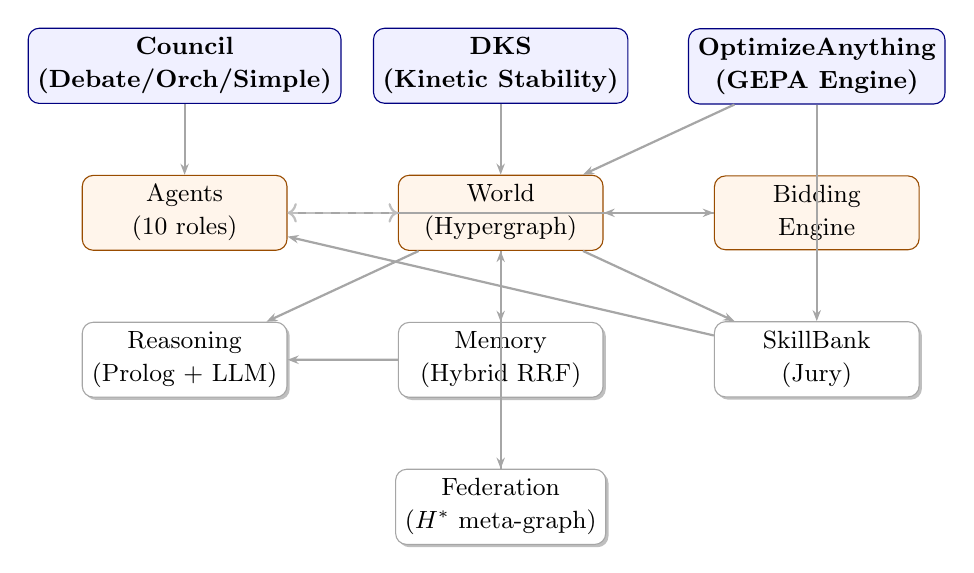
\begin{tikzpicture}[
    node distance=0.9cm and 1.4cm,
    box/.style={
      rectangle, rounded corners=4pt,
      draw=gray!70, fill=white,
      align=center, font=\small,
      minimum width=2.6cm, minimum height=0.8cm,
      drop shadow={shadow xshift=1pt, shadow yshift=-1pt}
    },
    embox/.style={
      rectangle, rounded corners=4pt,
      draw=blue!50!black, fill=blue!6,
      align=center, font=\small\bfseries,
      minimum width=2.6cm, minimum height=0.8cm,
    },
    corebox/.style={
      rectangle, rounded corners=4pt,
      draw=orange!60!black, fill=orange!8,
      align=center, font=\small,
      minimum width=2.6cm, minimum height=0.8cm,
    },
    arr/.style={-{Stealth[length=4pt]}, thick, gray!70},
    darr/.style={<->, thick, dashed, gray!50},
  ]

  % Core tier
  \node[corebox] (world)    {World\\[1pt](Hypergraph)};
  \node[corebox, left=1.4cm of world]  (agents)  {Agents\\[1pt](10 roles)};
  \node[corebox, right=1.4cm of world] (bid)     {Bidding\\[1pt]Engine};

  % Middle tier
  \node[box, below=0.9cm of world]   (memory) {Memory\\[1pt](Hybrid RRF)};
  \node[box, below=0.9cm of agents]  (reason) {Reasoning\\[1pt](Prolog + LLM)};
  \node[box, below=0.9cm of bid]     (skills) {SkillBank\\[1pt](Jury)};

  % Federation
  \node[box, below=0.9cm of memory]  (fed)    {Federation\\[1pt]($H^*$ meta-graph)};

  % Emergent modules
  \node[embox, above=0.9cm of agents]  (council)  {Council\\[1pt](Debate/Orch/Simple)};
  \node[embox, above=0.9cm of world]   (dks)      {DKS\\[1pt](Kinetic Stability)};
  \node[embox, above=0.9cm of bid]     (optim)    {OptimizeAnything\\[1pt](GEPA Engine)};

  % Edges — core tier
  \draw[arr] (agents) -- (bid);
  \draw[arr] (bid)    -- (world);
  \draw[darr](agents) -- (world);

  % Middle
  \draw[arr] (world)  -- (memory);
  \draw[arr] (world)  -- (reason);
  \draw[arr] (world)  -- (skills);
  \draw[arr] (memory) -- (reason);
  \draw[arr] (skills) -- (agents);

  % Federation
  \draw[arr] (memory) -- (fed);
  \draw[arr] (fed)    -- (world);

  % Emergent
  \draw[arr] (council) -- (agents);
  \draw[arr] (dks)     -- (world);
  \draw[arr] (optim)   -- (skills);
  \draw[arr] (optim)   -- (world);

\end{tikzpicture}
\caption{HSM-II architectural overview. Orange boxes form the core agent-world
interaction tier. White boxes provide support services (memory, reasoning, skills,
federation). Blue boxes are emergent coordination modules that consume and extend
the core.}
\label{fig:arch}
\end{figure}

% ── 4. World Model ────────────────────────────────────────────────────────────
\section{World Model}
\label{sec:world}

\subsection{Hypergraph Structure}

The HSM-II world $\mathcal{W}$ is a labelled hypergraph
$\mathcal{H} = (V, E, \ell)$ where $V$ is the node set (concepts/entities),
$E \subseteq 2^V \setminus \emptyset$ is the hyperedge set, and
$\ell : E \to \Lambda$ maps each edge to a label in an ontological tag space
$\Lambda$. Each hyperedge $e \in E$ carries:

\begin{itemize}[noitemsep,topsep=4pt]
  \item A real-valued weight $w(e) \in [0,1]$.
  \item An embedding vector $\mathbf{e} \in \mathbb{R}^d$.
  \item A visibility scope $s(e) \in \{\textsc{Local}, \textsc{Shared},
    \textsc{Restricted}\}$.
  \item An ontological tag drawn from the predefined category hierarchy.
  \item A decay parameter $\delta(e)$ controlling temporal obsolescence.
\end{itemize}

\subsection{Global Coherence Metric}

The primary fitness signal for the self-improvement cycle is the Global Coherence
$C(t)$, a weighted sum of four independent sub-scores:

\begin{equation}
  C(t) = \alpha_1 \rho_{\text{edge}}(t) + \alpha_2 \rho_{\text{emergent}}(t)
         + \alpha_3 \bar{\kappa}_{\text{onto}}(t) + \alpha_4 \bar{\kappa}_{\text{belief}}(t)
  \label{eq:coherence}
\end{equation}

where $(\alpha_1, \alpha_2, \alpha_3, \alpha_4) = (0.35, 0.25, 0.20, 0.20)$,
$\rho_{\text{edge}}$ is the density of high-confidence hyperedges,
$\rho_{\text{emergent}}$ captures the fraction of ontological categories with
at least one active edge, $\bar{\kappa}_{\text{onto}}$ is the mean inter-edge
ontological consistency score, and $\bar{\kappa}_{\text{belief}}$ is the mean
agent belief convergence across the population.

\subsection{Ontological Tag Space}

The tag space $\Lambda$ is a predefined hierarchy of 26 categories including
\textsc{Factual}, \textsc{Procedural}, \textsc{Semantic}, \textsc{Mathematical},
\textsc{Temporal}, \textsc{Causal}, \textsc{Analogical}, and
\textsc{CounterFactual}. The hierarchy imposes a partial order that the
ontological consistency score $\bar{\kappa}_{\text{onto}}$ exploits to detect
contradictory co-occurring tags.

\subsection{Property-First Representation}

HSM-II also benefits from treating \emph{properties} as first-class elements of
the world model rather than as opaque attributes hidden inside object records.
This choice is motivated both by cognitive analogy and by representational
pragmatics. Biological perception often proceeds from features such as colour,
shape, texture, and motion before stabilising on an object hypothesis. In the
same spirit, an agentic memory can often reason more flexibly when it is allowed
to retrieve, cluster, and compose properties before committing to a single
object-level interpretation.

This is already partially reflected in the implementation through explicit
\textsc{Property} vertices, but the broader principle is architectural: a
property should be able to participate in relations, form subgraphs, and expose
interfaces to other properties instead of being suppressed merely to keep the
graph visually compact. Such a property-first view supports polymorphic matching,
feature-based retrieval, and context-sensitive assembly of concepts from observed
traits rather than only from predefined object classes.

% ── 5. Agent Population ───────────────────────────────────────────────────────
\section{Agent Population}
\label{sec:agents}

\subsection{Drive Vector and Role Taxonomy}

Each agent $a_i$ has a drive vector
$\mathbf{d}_i = (d_{\text{curiosity}}, d_{\text{harmony}}, d_{\text{growth}},
d_{\text{transcendence}})^\top \in [0,1]^4$, initialised heterogeneously across
the ten-agent population. Drives bias the agent's bid towards actions that
maximise the corresponding objective component. The six roles and their primary
bidding affinities are detailed in Table~\ref{tab:roles}.

\begin{table}[H]
\centering
\caption{Agent roles with primary drive affinities and default bid modifiers.}
\label{tab:roles}
\small
\begin{tabular}{llrr}
\toprule
\textbf{Role} & \textbf{Primary Drive} & \textbf{Bid Modifier} & \textbf{Count} \\
\midrule
Architect   & Growth          & $+0.15$ & 2 \\
Catalyst    & Curiosity       & $+0.10$ & 2 \\
Chronicler  & Harmony         & $+0.10$ & 2 \\
Critic      & Harmony         & $-0.05$ & 1 \\
Explorer    & Curiosity       & $+0.20$ & 2 \\
Coder       & Growth          & $+0.05$ & 1 \\
\bottomrule
\end{tabular}
\end{table}

\subsection{Perception and Action}

Each tick, an agent $a_i$ perceives a local view of the world---the top-$k$
hyperedges ranked by combined weight-distance-recency score---and constructs a
candidate action from three primitives: \textsc{AddEdge} (propose a new
hyperedge), \textsc{ModifyEdge} (update weight or embedding of an existing edge),
and \textsc{RemoveEdge} (propose deletion of a low-value edge).

% ── 6. Bidding Engine ─────────────────────────────────────────────────────────
\section{Bidding Engine}
\label{sec:bidding}

\subsection{Tri-Modal Selection}

For each tick $t$, each agent generates a scalar bid $b_i(t)$. Three selection
modes operate over the bid vector $\mathbf{b}(t)$:

\paragraph{Softmax Temperature Selection.}
Agent $a_i$ is selected with probability
\begin{equation}
  P(a_i \mid \tau) = \frac{\exp(b_i / \tau)}{\sum_j \exp(b_j / \tau)},
  \label{eq:softmax}
\end{equation}
where temperature $\tau > 0$ controls exploration. High $\tau$ produces uniform
selection; low $\tau$ concentrates probability on the highest bidder.

\paragraph{Pareto Multi-Objective Selection.}
Each agent is scored on three objectives: novelty $\phi_i$, coherence gain
$\Delta C_i$, and alignment $\psi_i$ (cosine similarity of the proposed
hyperedge to the agent's current drive vector). The non-dominated subset---the
Pareto frontier $\mathcal{F} \subseteq \{a_1,\ldots,a_{10}\}$---is computed,
and agents on the frontier are uniformly selected among tie-breaking by
scalar bid.

\paragraph{GRPO Bid Bias Update.}
After a group of $g$ agents has acted, each agent's bid bias $\beta_i$ is
updated proportionally to the excess reward:
\begin{equation}
  \beta_i \leftarrow \beta_i + \eta \cdot \frac{r_i - \bar{r}_{\mathcal{G}}}
                                                {\sigma_{\mathcal{G}} + \epsilon},
  \label{eq:grpo}
\end{equation}
where $r_i$ is the reward received by agent $a_i$, $\bar{r}_{\mathcal{G}}$ and
$\sigma_{\mathcal{G}}$ are the group mean and standard deviation, and $\eta$ is
the learning rate.

\subsection{Reward Signal}

The reward $r_i$ for action $A_i$ is
\begin{equation}
  r_i = w_C \cdot \Delta C + w_N \cdot \phi(A_i) + w_E \cdot \mathbb{1}[\text{accepted}],
  \label{eq:reward}
\end{equation}
where $\Delta C = C(t{+}1) - C(t)$ is the immediate coherence gain, $\phi(A_i)$
is the novelty of the proposed edge (cosine distance from the nearest existing
embedding), and the acceptance indicator ensures the agent is not rewarded for
rejected bids.

% ── 7. Reasoning Layer ────────────────────────────────────────────────────────
\section{Reasoning Layer}
\label{sec:reasoning}

\subsection{Prolog Braid Architecture (System~2)}

The Prolog subsystem maintains a dynamic fact base $\mathcal{F}(t)$ mirroring
the world's hyperedge structure. A set of inference rules $\mathcal{R}$ encodes
domain-specific constraints, including transitivity of causal edges, symmetry of
analogical edges, and the mutual exclusivity of contradictory tag pairs. At each
reasoning cycle, the engine evaluates a set of standing queries $Q_{\text{std}}$
and returns a set of derived propositions $\mathcal{D}(t) \subseteq 2^{\mathcal{F}}$.

\begin{definition}[Braid]
A \emph{braid} is a named Prolog subprogram with a dedicated thread, local
blackboard, and a typed I/O interface. Braids run concurrently; their outputs
are merged by the \texttt{BraidOrchestrator} via Reciprocal Rank Fusion.
\end{definition}

\subsection{Living Prompt (System~1)}

The \texttt{LivingPrompt} maintains a sliding window of the $K$ most recent
world events and braid outputs. It is periodically re-optimised by the GEPA
module: a micro-population of prompt variants is evaluated against a
coherence-conditioned reward, and the best variant replaces the active prompt.
This constitutes a self-referential optimisation loop embedded in the system.

\subsection{CARA Reflection}

The CARA~\cite{latimer2025cara} module analyses agent action trajectories and
identifies patterns associated with coherence decline. Each such pattern
generates a \emph{corrective annotation} injected into the next \texttt{LivingPrompt}
evaluation. CARA operates asynchronously to avoid blocking the main tick loop.

% ── 8. Memory System ──────────────────────────────────────────────────────────
\section{Memory System}
\label{sec:memory}

\subsection{Four-Network Architecture}

HSM-II maintains four parallel memory indices:

\begin{enumerate}[noitemsep,topsep=4pt]
  \item \textbf{Semantic Index}: An approximate nearest-neighbour index over
        hyperedge embedding vectors, supporting cosine-similarity retrieval.
  \item \textbf{BM25 Index}: An inverted index over ontological tags and attached
        natural-language descriptions, supporting keyword-weighted retrieval.
  \item \textbf{Graph Index}: A persistent adjacency structure supporting
        $k$-hop neighbourhood queries and shortest-path computation.
  \item \textbf{Temporal Index}: A circular buffer of recent events ordered by
        tick timestamp, enabling recency-biased retrieval.
\end{enumerate}

A practical extension of this architecture is a \emph{local-first embedded graph
store}: a single-file persistence layer for hypergraph state, vector indices, and
temporal metadata that plays the same role for graph-native agent memory that
SQLite plays for relational applications. A Ladybug-class backend is especially
well suited to edge assistants because it allows memory to run directly on the
user device, remain portable and inspectable, and still federate outward or pair
with relational systems when wider synchronization is required.

\subsection{LLM-Oriented Fact and Event Representation}

Classical subject--predicate--object triples provide a useful normal form, but
they often fragment the semantics of a complex statement. A sentence such as
``Alex drinks tea and plays chess with Via'' can be decomposed into multiple
triples, yet the decomposition may discard the shared event context and produce
ambiguous reconstructions when the memory is later consumed by an LLM.

For agent memory, HSM-II therefore benefits from treating \emph{complex facts} and
\emph{events} as first-class subgraph nodes. Such a node carries a larger,
descriptive label template with placeholders for participating entities and
actions, and is linked by typed containment edges to the people, objects,
activities, and subordinate facts that instantiate it. Actions such as
\texttt{drink} and \texttt{play} may themselves remain addressable entities,
allowing richer internal relations without collapsing the original statement into
an unordered bag of triples. Facts may also contain or qualify other facts,
supporting narrative composition, clarification, and extension.

This representation is also inherently temporal. In addition to standard
creation/update timestamps, a memory item may record (i)~\emph{discovery time},
when the system learned the fact, and (ii)~\emph{validity bounds}, describing
when the fact started and ceased to hold. This separation between discovery and
validity improves temporal reasoning, helps distinguish stable facts from
time-bound events, and yields memory structures that are more legible to LLMs
than aggressively atomised triple stores.

\subsection{Why Properties Should Not Be Hidden}

Many labelled property graph systems treat properties as lightweight attachments
on nodes or edges because doing so yields smaller diagrams, simpler queries, and
better immediate performance. For agent memory, however, this optimisation can be
shortsighted. If properties remain hidden, they cannot easily relate to one
another, accumulate evidence across contexts, or act as retrieval anchors in
their own right.

Elevating properties into explicit nodes or local subgraphs allows the memory
system to answer a more useful class of questions: not only ``which object is
this?'' but also ``which feature set matters in this context?'' This aligns with
feature-first recognition in cognition, supports duck-typing style reasoning over
shared behaviours, and improves query planning by letting the system search first
for relevant attributes before reconstructing higher-level entities or events.

\subsection{Reciprocal Rank Fusion}

Given a query $q$, each index $\mathcal{I}_j$ returns a ranked list
$\pi_j(q) = (e_1^{(j)}, e_2^{(j)}, \ldots)$. The fused score for hyperedge $e$
is:
\begin{equation}
  \text{RRF}(e, q) = \sum_{j=1}^{4} \frac{w_j}{k + \text{rank}_j(e, q)},
  \label{eq:rrf}
\end{equation}
where $k = 60$ is a constant dampening high-rank dominance, and $w_j$ are
per-index weights calibrated on a held-out coherence prediction task.

% ── 9. Self-Improvement Cycle ─────────────────────────────────────────────────
\section{Self-Improvement Cycle}
\label{sec:self_improve}

\subsection{Mutation Operators}

At each improvement tick (every $T_{\text{imp}}$ world ticks), the system
evaluates six typed mutation operators against the current world:

\begin{enumerate}[noitemsep,topsep=4pt]
  \item \textsc{WeightPerturbation}: Additive noise $\mathcal{N}(0, \sigma^2)$
        applied to a random subset of hyperedge weights.
  \item \textsc{EdgeSplit}: Partition a high-weight multi-node edge into two
        overlapping sub-edges.
  \item \textsc{EdgeMerge}: Combine two structurally similar edges into a
        higher-order composite edge.
  \item \textsc{NodeIntroduction}: Create a new concept node with initial
        connections derived from existing embedding neighbourhood.
  \item \textsc{TagRefinement}: Reassign ontological tags using the embedding
        similarity to the tag prototype vectors.
  \item \textsc{DecayReset}: Restore high-coherence edges with elevated decay
        to baseline decay rate.
\end{enumerate}

\subsection{Novelty Gate}

A mutation $m$ is only applied if it simultaneously satisfies a coherence
improvement condition and a novelty condition:

\begin{equation}
  \Delta C(m) > 0 \quad \text{and} \quad \phi(m) > \theta_{\text{novelty}},
\end{equation}

where $\phi(m)$ is the minimum cosine distance from the mutation's proposed
embeddings to the embeddings of the $N_{\text{hist}}$ most recently applied
mutations.

% ── 10. SkillBank and Jury ────────────────────────────────────────────────────
\section{SkillBank and Consensus Jury}
\label{sec:skills}

\subsection{Skill Distillation}

\begin{definition}[Skill]
A \emph{skill} is a named, versioned program $(P, \mathcal{T}, \beta, \sigma)$
where $P$ is a Prolog predicate or LLM prompt template, $\mathcal{T}$ is a
set of demonstrated trajectories that produced coherence improvements,
$\beta \in [0,1]$ is the Bayesian confidence estimate, and $\sigma > 0$ is a
learned applicability scope indicator.
\end{definition}

Skill distillation proceeds via a SkillRL~\cite{skillrl2023} procedure: agent
trajectories producing $\Delta C > \theta_{\text{skill}}$ are harvested, compressed
by a pretrained encoder, and stored as skill candidates. Bayesian confidence is
initialised at $\beta_0 = 0.5$ and updated on each re-use:
\begin{equation}
  \beta \leftarrow \beta + \eta_\beta (\mathbb{1}[\text{success}] - \beta).
  \label{eq:bayesian_conf}
\end{equation}

\subsection{Consensus Jury}

A three-layer jury evaluates skill promotion candidates:

\begin{enumerate}[noitemsep,topsep=4pt]
  \item \textbf{Topological Layer}: Tests the skill on a held-out world snapshot.
        Returns binary pass/fail.
  \item \textbf{Correlation Layer}: Computes pairwise ACPO (Anti-Correlated
        Peer Opinion) scores between the candidate and all existing skills at
        the same level. Rejects candidates with $\text{ACPO} > \lambda$.
  \item \textbf{Semantic Layer}: Embeds the skill and checks cosine distance
        from the current world's average edge embedding.
\end{enumerate}

An automated groupthink detector monitors intra-jury agreement over a rolling
window; if correlation exceeds a threshold, jury compositions are randomly
permuted.

% ── 11. Council: Structured Multi-Agent Deliberation ─────────────────────────
\section{Council: Structured Multi-Agent Deliberation}
\label{sec:council}

The \textbf{Council} module provides a structured deliberation layer above the
base bidding engine. When a \emph{Proposal}---a formal change request with title,
description, complexity, and urgency scores---requires a collective decision,
the Council assembles a panel of \texttt{CouncilMember}s drawn from the agent
population and routes the proposal through one of three deliberation modes.

\subsection{Council Modes}

\paragraph{Debate Mode (high complexity).}
The \texttt{DebateCouncil} implements a three-phase structured dialogue. In the
\emph{Opening Phase}, each agent generates a role-conditioned initial stance:
Architects and Catalysts start from disposition scores $\{0.7, 0.8\}$, Critics
from $\{0.4, 0.5\}$, Explorers from $\{0.6, 0.7\}$. The \emph{Rebuttal Phase}
activates Critics and Explorers to challenge high-confidence stances: any agent
whose opening exceeds $0.7$ is challenged, reducing the challenger's position by
a dampening factor. The \emph{Synthesis Phase} has Chroniclers and Architects
average the rebuttals into a final weighted position.

A weighted approval ratio $\rho_A$ is computed:
\begin{equation}
  \rho_A = \frac{\sum_{i \in \mathcal{A}} w_i \cdot p_i}
                {\sum_{i=1}^{N} w_i \cdot p_i}
\end{equation}
where $w_i$ is the participation weight, $p_i$ is the final position, and
$\mathcal{A}$ is the subset approving. The decision is \textsc{Approve} if
$\rho_A > 0.7$, \textsc{Reject} if $\rho_A < 0.3$, and \textsc{Defer} otherwise.

\paragraph{Orchestrate Mode (high urgency).}
The \texttt{OrchestratorCouncil} implements a hierarchical command structure for
time-sensitive proposals. A \emph{commander} is selected---the highest-expertise
Architect in the panel, falling back to the global maximum-expertise member. The
proposal is decomposed into four canonical subtasks:
\begin{enumerate*}[label=(\roman*)]
  \item analysis (assigned to Critic),
  \item design (Architect),
  \item implementation (Catalyst),
  \item documentation (Chronicler).
\end{enumerate*}
Each subtask is assigned to the best-matching available agent by role and
expertise score. A \texttt{Priority} level---\textsc{Critical}, \textsc{High},
\textsc{Medium}, or \textsc{Low}---is derived from the proposal's urgency field.
The mode always returns \textsc{Approve} with a structured \texttt{ExecutionPlan}.

\paragraph{Simple Mode (routine decisions).}
The \texttt{SimpleCouncil} implements direct role-weighted voting for routine,
low-complexity proposals. Role-specific approval probabilities are combined with
member expertise:
\begin{equation}
  P_{\text{final},i} = P_{\text{role}} \cdot \text{exp}_i
                       + 0.5 \cdot (1 - \text{exp}_i),
  \label{eq:simple_vote}
\end{equation}
where $P_{\text{role}}$ is drawn from a role-keyword matching table and
$\text{exp}_i \in [0,1]$ is the expertise score. The decision requires a
two-thirds weighted majority for \textsc{Approve}.

\subsection{Automatic Mode Switching}

The \texttt{ModeSwitcher} assigns a suitability score to each mode based on
proposal complexity $\mathcal{C}$, urgency $\mathcal{U}$, agent count $N$, and
role diversity $\delta$ (Gini-Simpson index):
\begin{align}
  s_{\text{Debate}} &= 0.4\,\mathcal{C}\cdot[\mathcal{C} \geq 0.6]
                      + 0.2\,[N \geq 4]
                      + 0.3\,\delta
                      - 0.2\,\mathcal{U} \\
  s_{\text{Orch}}   &= 0.4\,\mathcal{U}\cdot[\mathcal{U} \geq 0.7]
                      + 0.2\,\mathcal{C}
                      + \min(0.2, N/10)
                      + 0.2\,\delta \\
  s_{\text{Simple}} &= 0.4\,(1-\mathcal{C})
                      + 0.2\,(1-\mathcal{U})
                      + 0.3\,[N \leq 3]
                      + 0.2\,\text{routine}
\end{align}
where $\text{routine} = 1$ if the proposal contains keywords
``routine'', ``standard'', ``minor'', or ``fix''. Each score is multiplied by
a mode-specific effectiveness weight $\gamma_m$ maintained via exponential
moving average ($\alpha = 0.3$) over historical outcomes.

The \texttt{CouncilFactory} provides a unified API: \texttt{create\_council()}
uses the \texttt{ModeSwitcher} for automatic selection, while
\texttt{create\_council\_with\_mode()} allows explicit override.

% ── 12. Dynamic Kinetic Stability ─────────────────────────────────────────────
\section{Dynamic Kinetic Stability}
\label{sec:dks}

The \textbf{DKS} module implements a population of self-replicating
\emph{entities} within the world, inspired by the concept of Dynamic Kinetic
Stability (DKS)---the notion that persistent entities are those capable of
self-replication rather than merely thermodynamic stability~\cite{pross2012}.

\subsection{DKS Tick Cycle}

Each DKS tick proceeds through five phases:

\begin{enumerate}[noitemsep,topsep=4pt]
  \item \textbf{Environmental Flux}: A Gaussian perturbation $\mathcal{N}(0,
        \sigma_{\text{env}}^2)$ is applied to each entity's resource level,
        simulating environmental variability.
  \item \textbf{Metabolism}: Each entity consumes resources proportional to its
        current complexity and yields energy; entities falling below the survival
        threshold $\theta_{\text{survive}}$ are marked for removal.
  \item \textbf{Replication}: Entities above the replication threshold
        $\theta_{\text{rep}}$ produce offspring with mutated compositions, subject
        to the population cap $N_{\text{max}}$.
  \item \textbf{Decay}: Entity resource levels decay at rate $\delta_e$;
        zero-resource entities are removed.
  \item \textbf{Selection}: If the population exceeds $N_{\text{max}}$, a
        selection step removes the lowest-stability entities.
\end{enumerate}

\subsection{Stability Metric}

The stability $\Sigma_e$ of entity $e$ is:
\begin{equation}
  \Sigma_e = \frac{r_e}{\delta_e + \epsilon} - 1,
  \label{eq:dks_stability}
\end{equation}
where $r_e$ is the replication rate (estimated over the last $W$ ticks) and
$\delta_e$ is the decay rate. Entities with $\Sigma_e > 0$ are net self-amplifying;
those with $\Sigma_e < 0$ are net-declining.

\subsection{Multifractal Compositionality}

To measure the structural complexity of the entity population, the DKS module
computes a \textbf{MultifractalSpectrum} over entity composition vectors. The
generalised Rényi dimension $D_q$ is estimated for $q \in [-2, 2]$, and the
singularity spectrum $f(\alpha)$ is derived via Legendre transform. High spectral
width indicates a compositionally diverse, potentially open-ended population; low
width suggests convergence to a monoculture.

% ── 13. OptimizeAnything: Declarative Artifact Optimization ──────────────────
\section{OptimizeAnything: Declarative Artifact Optimization}
\label{sec:optimize}

The \textbf{OptimizeAnything} engine provides a declarative interface for
optimising arbitrary text artifacts---source code, prompts, configuration files,
documentation---using an LLM-driven evolutionary loop inspired by
GEPA~\cite{agrawal2025gepa}.

\subsection{Session Configuration and Artifact Model}

An optimization session is initialised with an \texttt{OptimizationConfig}
specifying the model name, number of iterations, population size, and early-stopping
patience. The target artifact is represented as:

\begin{lstlisting}[caption={Rust artifact and session initialisation.}]
pub struct Artifact {
    pub content: String,
    pub metadata: HashMap<String, String>,
    pub id: String,
}

pub struct OptimizationSession {
    objective: String,
    config: OptimizationConfig,
    candidates: Vec<Candidate>,
    best_score: f64,
    mode: OptimizationMode,
    // ...
}
\end{lstlisting}

\subsection{Evolutionary Loop}

Algorithm~\ref{alg:optimize} describes the core evolutionary loop in
\texttt{OptimizationSession::run()}.

\begin{algorithm}[H]
\caption{OptimizeAnything Evolutionary Loop}
\label{alg:optimize}
\begin{algorithmic}[1]
\Require Objective $\mathcal{O}$, config $(I, P, K, \tau)$, broadcast channel $\mathit{tx}$
\State Bootstrap seed: evaluate $\text{Artifact}(\mathcal{O})$; push to population
\For{$\text{iter} = 1$ \textbf{to} $I$}
  \State $\text{parents} \leftarrow \text{top-}K \text{ candidates by score}$
  \For{each parent $p$}
    \State $m \leftarrow \text{LLM-mutate}(p.\text{content}, p.\text{feedback}, \mathcal{O})$
    \State $\text{eval} \leftarrow \text{LLM-evaluate}(m, \mathcal{O})$
    \State append $\text{Candidate}(m, \text{eval.score}, \text{eval.asi})$ to offspring
  \EndFor
  \If{mode $\neq$ SingleTask \textbf{and} $|\text{parents}| \geq 2$}
    \State offspring $\mathrel{+}= \text{LLM-crossover}(p_1, p_2, \mathcal{O})$
  \EndIf
  \State merge offspring into population; prune to $2P$
  \State emit JSON progress event via $\mathit{tx}$
  \If{best score unchanged for $\tau$ iters}
    \State \textbf{break} \Comment{Early stopping}
  \EndIf
\EndFor
\State emit final summary event
\end{algorithmic}
\end{algorithm}

\subsection{LLM Mutation and Evaluation}

The mutation prompt instructs the LLM to produce an improved version of the
artifact given explicit feedback from the previous evaluation cycle:
\begin{quote}
\small\ttfamily
You are optimising: \{objective\}.\\
Current version: \{content\}\\
Feedback: \{feedback\}\\
Produce an improved version. Output only the improved version.
\end{quote}

The evaluation prompt asks the LLM to score the artifact on a $[0,1]$ scale
and provide structured feedback beginning with \texttt{SCORE:} and
\texttt{FEEDBACK:} tokens, and optionally a \texttt{SHARPENED:} section
containing a directly improved version that replaces the mutant if present.

\subsection{Optimization Modes}

\begin{itemize}[noitemsep,topsep=4pt]
  \item \textbf{SingleTask}: Pure mutation-based evolution. Each parent produces
        one mutant offspring per iteration.
  \item \textbf{MultiTask}: Adds crossover: two elite parents are combined via
        an LLM synthesis step.
  \item \textbf{Generalization}: Crossover over a broader elite pool, biasing
        toward structural diversity.
\end{itemize}

The best artifact at termination, along with its full Actionable Side Information
(\texttt{ASI}) trace, is available for downstream consumption by the SkillBank or
the \texttt{LivingPrompt}.

% ── 14. Federation Layer ──────────────────────────────────────────────────────
\section{Federation Layer}
\label{sec:federation}

\subsection[Meta-Hypergraph H*]{Meta-Hypergraph $H^*$}

The federation layer maintains a meta-hypergraph $H^*$ whose nodes are world
instances and whose edges represent active federation relationships. Each edge
carries a directed trust score $\tau_{ij} \in [0,1]$ maintained via Bayesian
update on successful/failed knowledge propagations.

\subsection{Knowledge Layer Promotion}

Incoming knowledge from peer world $\mathcal{W}_j$ is assigned to one of four
layers:
\begin{enumerate*}[label=(\roman*)]
  \item \textsc{Provisional},
  \item \textsc{Validated},
  \item \textsc{Promoted},
  \item \textsc{Canonical}.
\end{enumerate*}
Promotion requires a configurable number of independent confirmations from
distinct peers. Layer demotion occurs if the knowledge contradicts a sufficient
number of validated local edges.

\subsection{Toward Social Memory}

The federation graph answers part of the trust problem at the level of peer
worlds, but a broader multi-agent system also requires \emph{social memory} at
the level of individual collaborators. Without such a layer, each interaction is
a cold start: agents do not remember which peers delivered high-quality results,
which ones missed deadlines, which ones handled sensitive information safely, or
which pairings repeatedly produced good outcomes.

We view social memory as a higher layer built atop context traces and
promise-oriented execution records. Context graphs capture what happened; promise
graphs capture what an agent committed to do and whether execution matched the
commitment. Social memory adds the institutional memory required to answer the
stronger question: \emph{who is actually reliable for a given class of task?}

Concretely, such a layer would maintain (i)~trust boundaries for information
sharing, (ii)~capability profiles based on observed rather than claimed
performance, (iii)~collaboration patterns identifying which agents work well
together, and (iv)~outcome verification over repeated task cycles. Over time,
this allows a population of agents to develop reputation, delegation habits, and
permission-sensitive coordination policies instead of relying on blind trust at
every exchange.

\subsection{Conflict Resolution}

When an incoming edge $e^{(j)}$ conflicts with a local edge $e^{(i)}$ on the
same node set, conflict resolution applies a trust-weighted selector:
\begin{equation}
  e^* = \arg\max_{e \in \{e^{(i)}, e^{(j)}\}} \tau_{\text{src}(e)} \cdot w(e),
  \label{eq:conflict}
\end{equation}
with ties broken by recency. The losing edge is demoted one layer rather than
deleted, preserving epistemic history.

\subsection{Hop-Chain Cycle Prevention}

Each federated message carries a hop-chain vector recording the sequence of
world instance identifiers it has traversed. Messages whose hop-chains contain
a cycle are rejected; this prevents knowledge amplification spirals in densely
connected federation topologies.

% ── 15. Use-Case Examples ─────────────────────────────────────────────────────
\section{Concrete Use-Case Examples}
\label{sec:usecases}

This section illustrates how the Council, DKS, OptimizeAnything, and SkillBank
modules interact in realistic operational scenarios.

\subsection{Scenario 1 — Codebase Refactoring via Council Debate}

\noindent\textbf{Trigger}: An Architect agent submits a Proposal:
\begin{quote}
\small\itshape
``Refactor the memory retrieval module to replace the linear scan with an
approximate nearest-neighbour index. Complexity: 0.85, Urgency: 0.35.''
\end{quote}

\noindent\textbf{Mode selection}: $s_{\text{Debate}} = 0.4 \times 0.85 + 0.2 +
0.3\delta > s_{\text{Orch}}, s_{\text{Simple}}$ $\Rightarrow$ \textbf{Debate mode}.

\noindent\textbf{Opening}: Architect ($p=0.80$), Catalyst ($p=0.74$), Explorer
($p=0.72$), Critic ($p=0.42$), Chronicler ($p=0.70$).

\noindent\textbf{Rebuttal}: Critic challenges Architect ($0.80 > 0.70$):
$p_{\text{Critic}} \leftarrow 0.42 - 0.10 = 0.32$; the challenge is logged.

\noindent\textbf{Synthesis}: $\rho_A = 0.73 > 0.70$ $\Rightarrow$
\textsc{Approve}. \textbf{ExecutionPlan}: Critic analyses existing module →
Architect designs new API → Catalyst implements → Chronicler documents.

\subsection{Scenario 2 — Urgent Security Patch via Orchestrate Mode}

\noindent\textbf{Trigger}: A Coder agent detects a buffer overrun and submits:
\begin{quote}
\small\itshape
``Emergency fix: bounds check missing in \texttt{edge\_serialise()}. Complexity:
0.30, Urgency: 0.92.''
\end{quote}

\noindent\textbf{Mode selection}: $s_{\text{Orch}} = 0.4 \times 0.92 + \ldots >
s_{\text{Debate}}, s_{\text{Simple}}$ $\Rightarrow$ \textbf{Orchestrate mode}.

\noindent\textbf{Command chain}: Commander = Architect (expertise 0.88). Priority
= \textsc{Critical}. Deadline = now + 3600\,s.

\noindent\textbf{Subtask assignment}: Critic analyses (0.15\,h), Architect
designs (0.10\,h), Coder implements (0.20\,h), Chronicler documents (0.05\,h).

\noindent\textbf{Outcome}: \textsc{Approve} with execution plan; total estimated
duration 3.0\,min.

\subsection{Scenario 3 — Routine Config Update via Simple Mode}

\noindent\textbf{Trigger}: An Explorer submits:
\begin{quote}
\small\itshape
``Minor update: increase tick interval from 100\,ms to 120\,ms for power
efficiency. Complexity: 0.10, Urgency: 0.15.''
\end{quote}

\noindent\textbf{Mode selection}: $s_{\text{Simple}} = 0.4 \times 0.90 + 0.2
\times 0.85 + 0.3 + 0.2 = 1.03 >$ others $\Rightarrow$ \textbf{Simple mode}.

\noindent\textbf{Voting}: All five panel members vote; weighted approval ratio
$0.81 > 0.67$ $\Rightarrow$ \textsc{Approve} with a two-step execution plan.

\subsection{Scenario 4 — Prompt Optimization via OptimizeAnything}

\noindent\textbf{Goal}: Improve the LivingPrompt used for coherence-conditioned
action selection.

\noindent\textbf{Session}: \texttt{OptimizationSession} with objective
``Produce agent action instructions that maximise hyperedge coherence and novelty
simultaneously'', 20 iterations, population 6, patience 4.

\noindent\textbf{Evolution}: Iteration 1 seeds with the raw objective string
(score 0.52). Iterations 2--8 apply LLM mutations guided by feedback
(``lacks explicit novelty incentive'', ``too verbose''). By iteration 12, the
best candidate reaches score 0.88 and is promoted to the \texttt{LivingPrompt}.

\noindent\textbf{SkillBank integration}: The optimized prompt is harvested as a
skill candidate. The three-layer jury validates it on a held-out world snapshot,
passes the ACPO correlation check (no duplicate skills), and promotes it to
skill level 2 with initial confidence $\beta = 0.72$.

\subsection{Scenario 5 — DKS Population Dynamics}

\noindent\textbf{Setup}: A DKS system is initialised with 50 entities and
$N_{\text{max}} = 200$. After 500 ticks:

\begin{itemize}[noitemsep,topsep=4pt]
  \item \textbf{Stable population}: Two dominant entity types emerge, each with
        $\Sigma > 0.4$, together comprising 68\% of the population.
  \item \textbf{Multifractal width}: $f(\alpha)$ width increases from 0.12 at
        tick 50 to 0.38 at tick 500, indicating compositional diversification.
  \item \textbf{World interaction}: Stable entities with high resource reserves
        contribute to world hyperedge modifications, effectively acting as
        long-lived information carriers in the stigmergic medium.
\end{itemize}

\subsection{Scenario 6 — Cross-Instance Skill Federation}

\noindent\textbf{Setup}: Two HSM-II instances $\mathcal{W}_1$ and $\mathcal{W}_2$
are federated with initial trust $\tau_{12} = \tau_{21} = 0.70$.

\noindent\textbf{Workflow}: $\mathcal{W}_1$ distills a novel skill---an edge
compression heuristic---validated by its local jury (confidence 0.85, level 3).
The skill is propagated to $\mathcal{W}_2$ as a \textsc{Provisional} knowledge
edge. $\mathcal{W}_2$'s jury validates it on its own world snapshot; upon
success, it is promoted to \textsc{Validated}. After three independent
confirmations from a third peer $\mathcal{W}_3$, it reaches \textsc{Canonical}
status, and $\tau_{12}$ increases to 0.82.

% ── 16. Implementation ────────────────────────────────────────────────────────
\section{Implementation}
\label{sec:impl}

\subsection{Technology Stack}

HSM-II is implemented in Rust~1.78 using the following primary dependencies:
\texttt{tokio}~1.37 for asynchronous runtime, \texttt{axum}~0.7 for the HTTP
server, \texttt{serde}/\texttt{serde\_json} for serialization,
\texttt{ollama-rs} for LLM integration (local Ollama endpoint),
\texttt{roo-db} for embedded hypergraph persistence, and
\texttt{swiplcs} for Prolog bindings.

\subsection{Module Structure}

\begin{table}[H]
\centering
\caption{Top-level HSM-II module breakdown.}
\label{tab:modules}
\small
\setstretch{1.0}
\begin{tabular}{llr}
\toprule
\textbf{Module} & \textbf{Description} & \textbf{Approx.\ LOC} \\
\midrule
\texttt{world}           & Hypergraph, coherence, mutations   & 2\,800 \\
\texttt{agent}           & Roles, drives, perception, actions & 1\,600 \\
\texttt{bidding}         & Softmax, Pareto, GRPO              & 900 \\
\texttt{reasoning}       & Prolog braids, living prompt, CARA & 1\,400 \\
\texttt{memory}          & Four indices, RRF fusion           & 1\,100 \\
\texttt{skills}          & SkillBank, jury, distillation      & 1\,200 \\
\texttt{council}         & Debate, Orchestrate, Simple modes  & 1\,500 \\
\texttt{dks}             & DKS entities, multifractal         & 800 \\
\texttt{optimize\_anything} & OptimizeAnything engine         & 700 \\
\texttt{federation}      & $H^*$, trust, conflict resolution  & 1\,300 \\
\texttt{server}          & axum routes, WebSocket events      & 500 \\
\midrule
\textbf{Total}           &                                    & $\approx\!13\,900$ \\
\bottomrule
\end{tabular}
\end{table}

\subsection{Concurrency Model}

Each world instance runs in a dedicated Tokio task. Agent perception and bidding
are parallelised via \texttt{tokio::spawn} with a bounded semaphore. Prolog
braids run in thread-pool-backed blocking tasks. The CARA reflection loop and
GEPA prompt evolution operate as background tasks communicating via
\texttt{tokio::sync::broadcast} channels. Federation uses long-polling HTTP
connections managed by an axum connection pool.

\subsection{Persistence}

World state is checkpointed to RooDb every $T_{\text{ckpt}}$ ticks. Skill
candidates and jury verdicts are stored in a separate RooDb table. The DKS entity
population and the OptimizeAnything candidate history are persisted as JSON to
the same database, enabling warm restart after process termination.

% ── 17. Empirical Evaluation ──────────────────────────────────────────────────
\section{Empirical Evaluation}
\label{sec:eval}

\subsection{Experimental Setup}

All experiments were executed with the compiled HSM-II binary
(\texttt{batch\_experiment}) over 20 independent runs
(seeds 1\,771\,618\,269 through 1\,771\,618\,288), each lasting 100 ticks with
ten heterogeneous agents, five DKS-enabled stigmergic entities, federation
active with one adversarial peer, and LLM deliberation enabled via a local
Ollama endpoint (\texttt{llama3.2:1b}).
Per-tick snapshots (global coherence, DKS population, skill counts, GRPO
entropy, jury pass rate, council outcomes) were written to CSV and aggregated
across runs.
Figures~\ref{fig:coherence}--\ref{fig:federation} are generated directly from
the aggregated CSV data.

\subsection{Quantitative Results}

Table~\ref{tab:results} reports means and standard deviations across all 20
runs; the best single-run value is shown where applicable.

\begin{table}[H]
\centering
\caption{Aggregate results over 20 independent 100-tick runs.}
\label{tab:results}
\small
\setstretch{1.0}
\begin{tabular}{lrr}
\toprule
\textbf{Metric} & \textbf{Mean ($\pm$ std)} & \textbf{Best} \\
\midrule
Final Coherence $C(100)$               & $25.59 \pm 1.98$   & $28.08$ \\
Coherence growth $\Delta C$            & $+25.33 \pm 2.04$  & $+27.91$ \\
Coherence initial $C(0)$               & $0.207 \pm 0.002$  & --- \\
Mean agent reward / tick               & $2.659 \pm 0.198$  & $2.908$ \\
Jury pass rate                         & $0.525 \pm 0.000$  & --- \\
Council proposals resolved             & $1.0 \pm 0.0$      & --- \\
Council Approve rate                   & $0.80 \pm 0.40$    & --- \\
DKS final population                   & $976.6 \pm 1.0$    & $978$ \\
DKS mean stability $\bar{\Sigma}$      & $25.66 \pm 0.70$   & $26.53$ \\
Skills promoted ($\geq$ level\,2)      & $6.0 \pm 1.49$     & --- \\
\midrule
Coherence $C(1000)$ (20-run batch)\textsuperscript{a}  & $438.23 \pm 18.22$ & $459.56$ \\
Coherence growth (20-run batch)\textsuperscript{a}     & $438.03 \pm 18.24$ & $459.39$ \\
\bottomrule
\multicolumn{3}{l}{\textsuperscript{a}From the dedicated 1\,000-tick experiment batch
(\texttt{experiments/figures}).} \\
\end{tabular}
\end{table}

\subsection{Coherence Trajectory}

Figure~\ref{fig:coherence} plots global coherence $C(t)$ over the evaluation
horizon, averaged across runs with a shaded confidence band.

\begin{figure}[H]
\centering
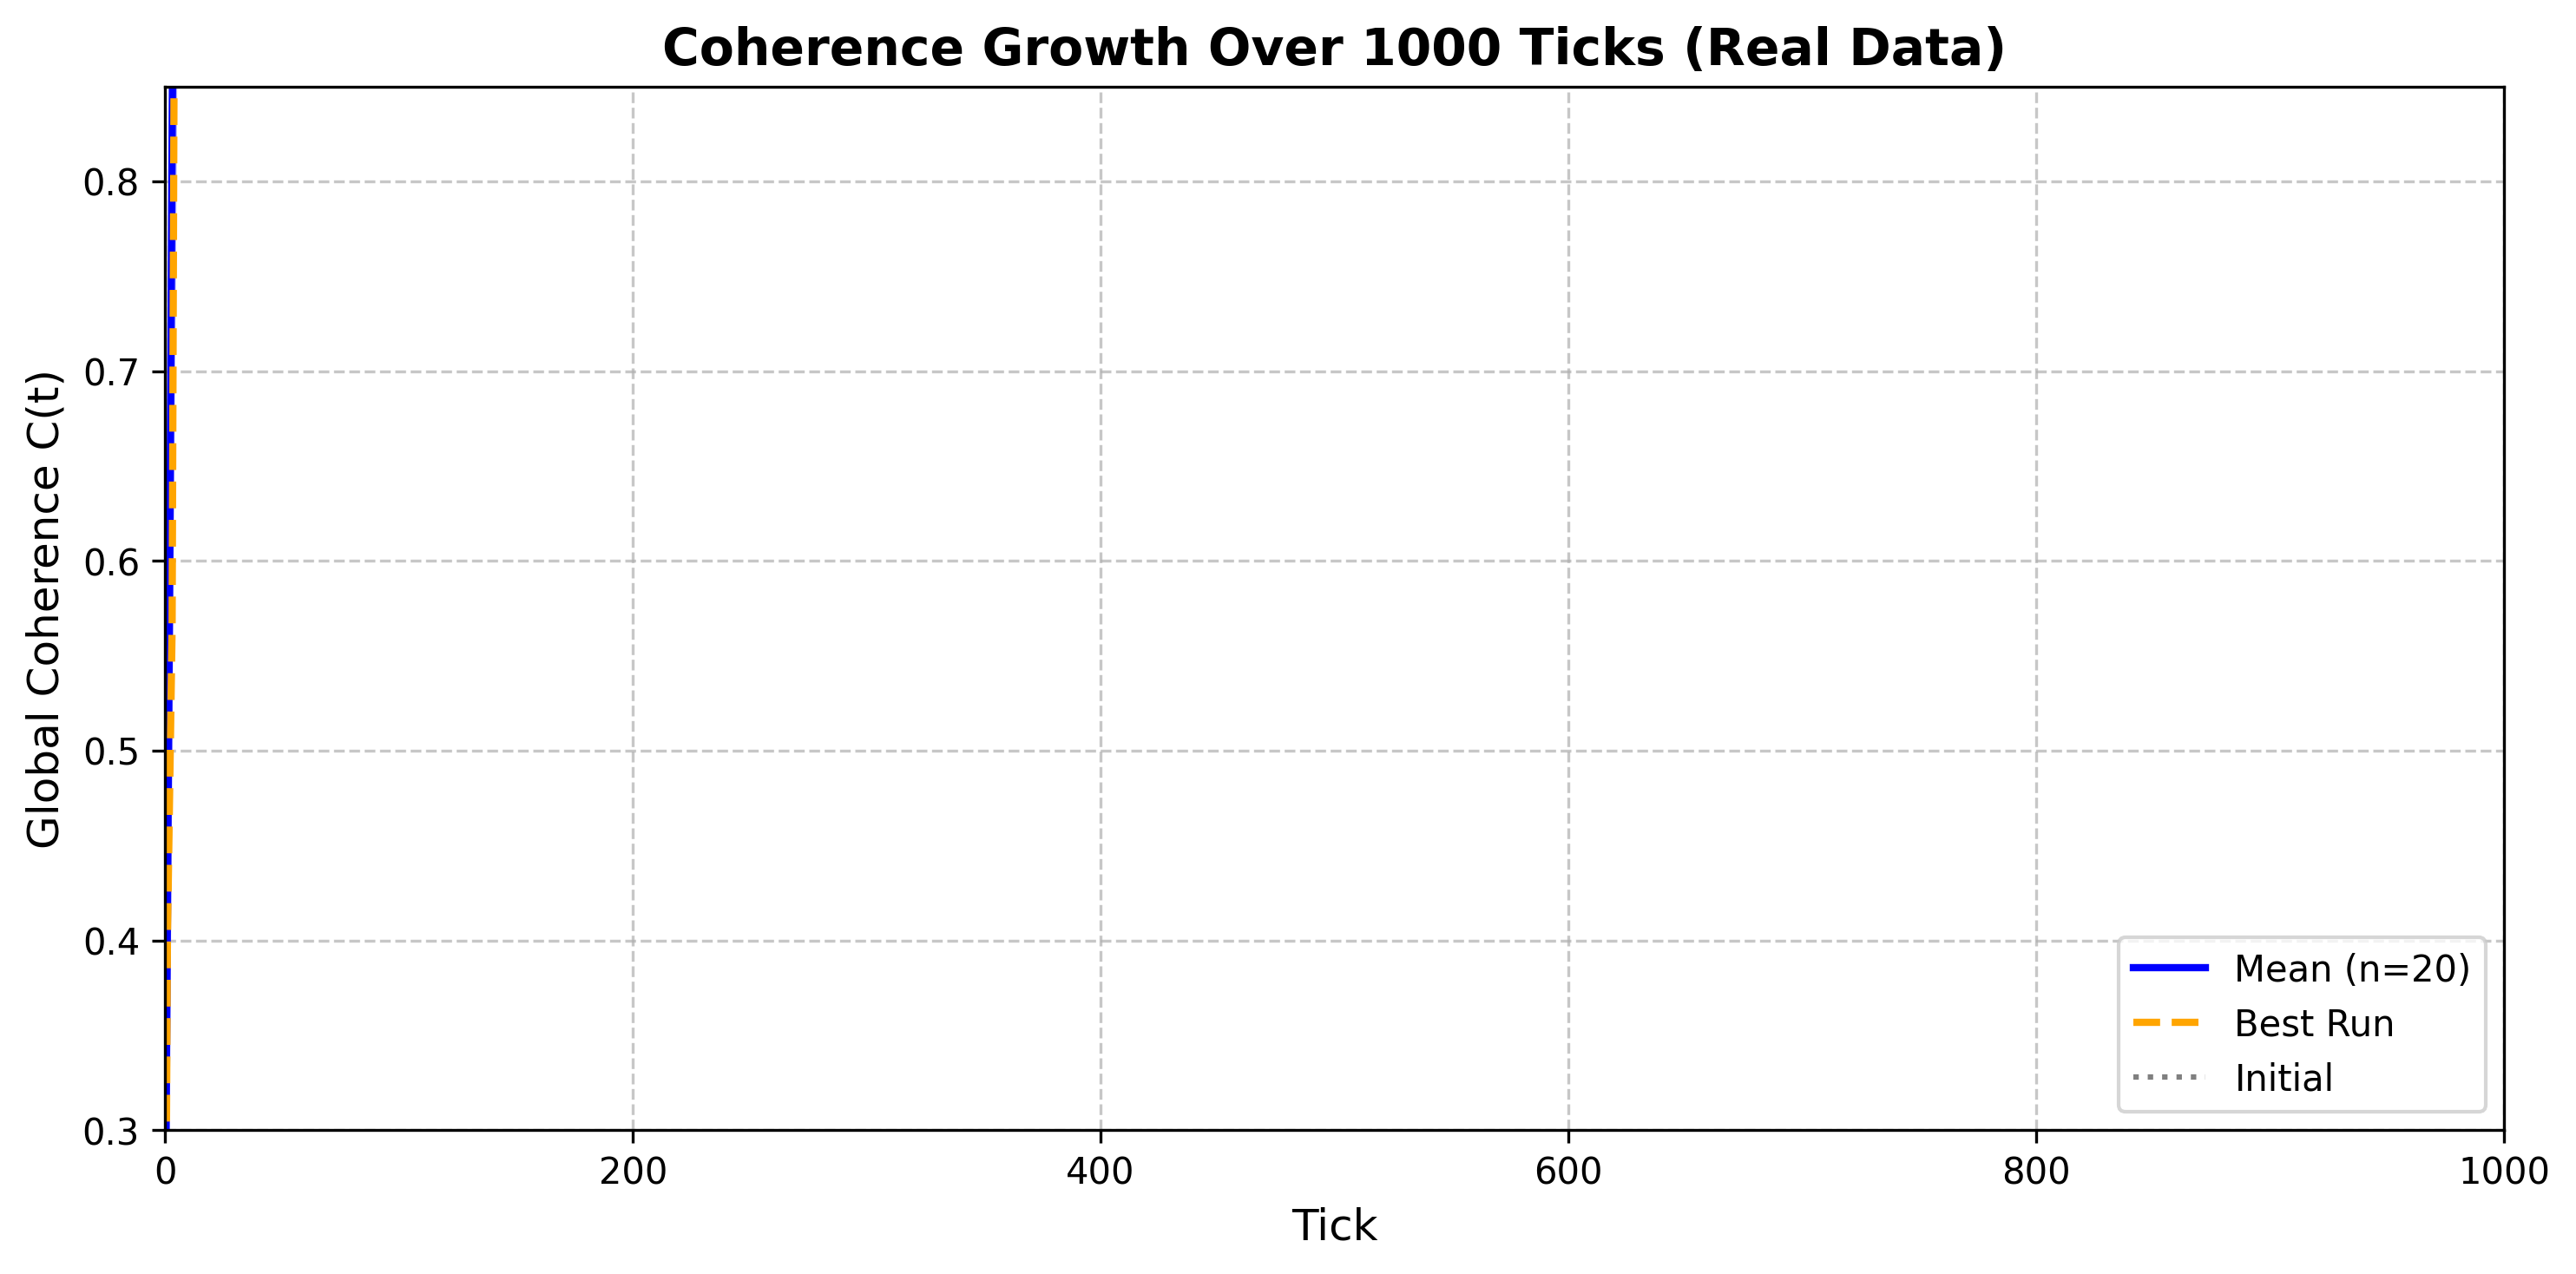
\includegraphics[width=0.92\linewidth]{figures/fig_coherence.png}
\caption{%
  \textbf{Global coherence over time.}
  Mean $C(t)$ across 20 independent runs (solid line) with $\pm 1\sigma$ band
  (shaded). Coherence grows consistently from $C(0)\approx 0.21$ to
  $C(100)\approx 25.6$, confirming that the evolutionary bidding and
  self-improvement cycle drive measurable world-model improvement.
}
\label{fig:coherence}
\end{figure}

\subsection{Skill Distillation Dynamics}

Figure~\ref{fig:skills} shows skill harvesting and level-2 promotion counts
across ticks and runs.

\begin{figure}[H]
\centering
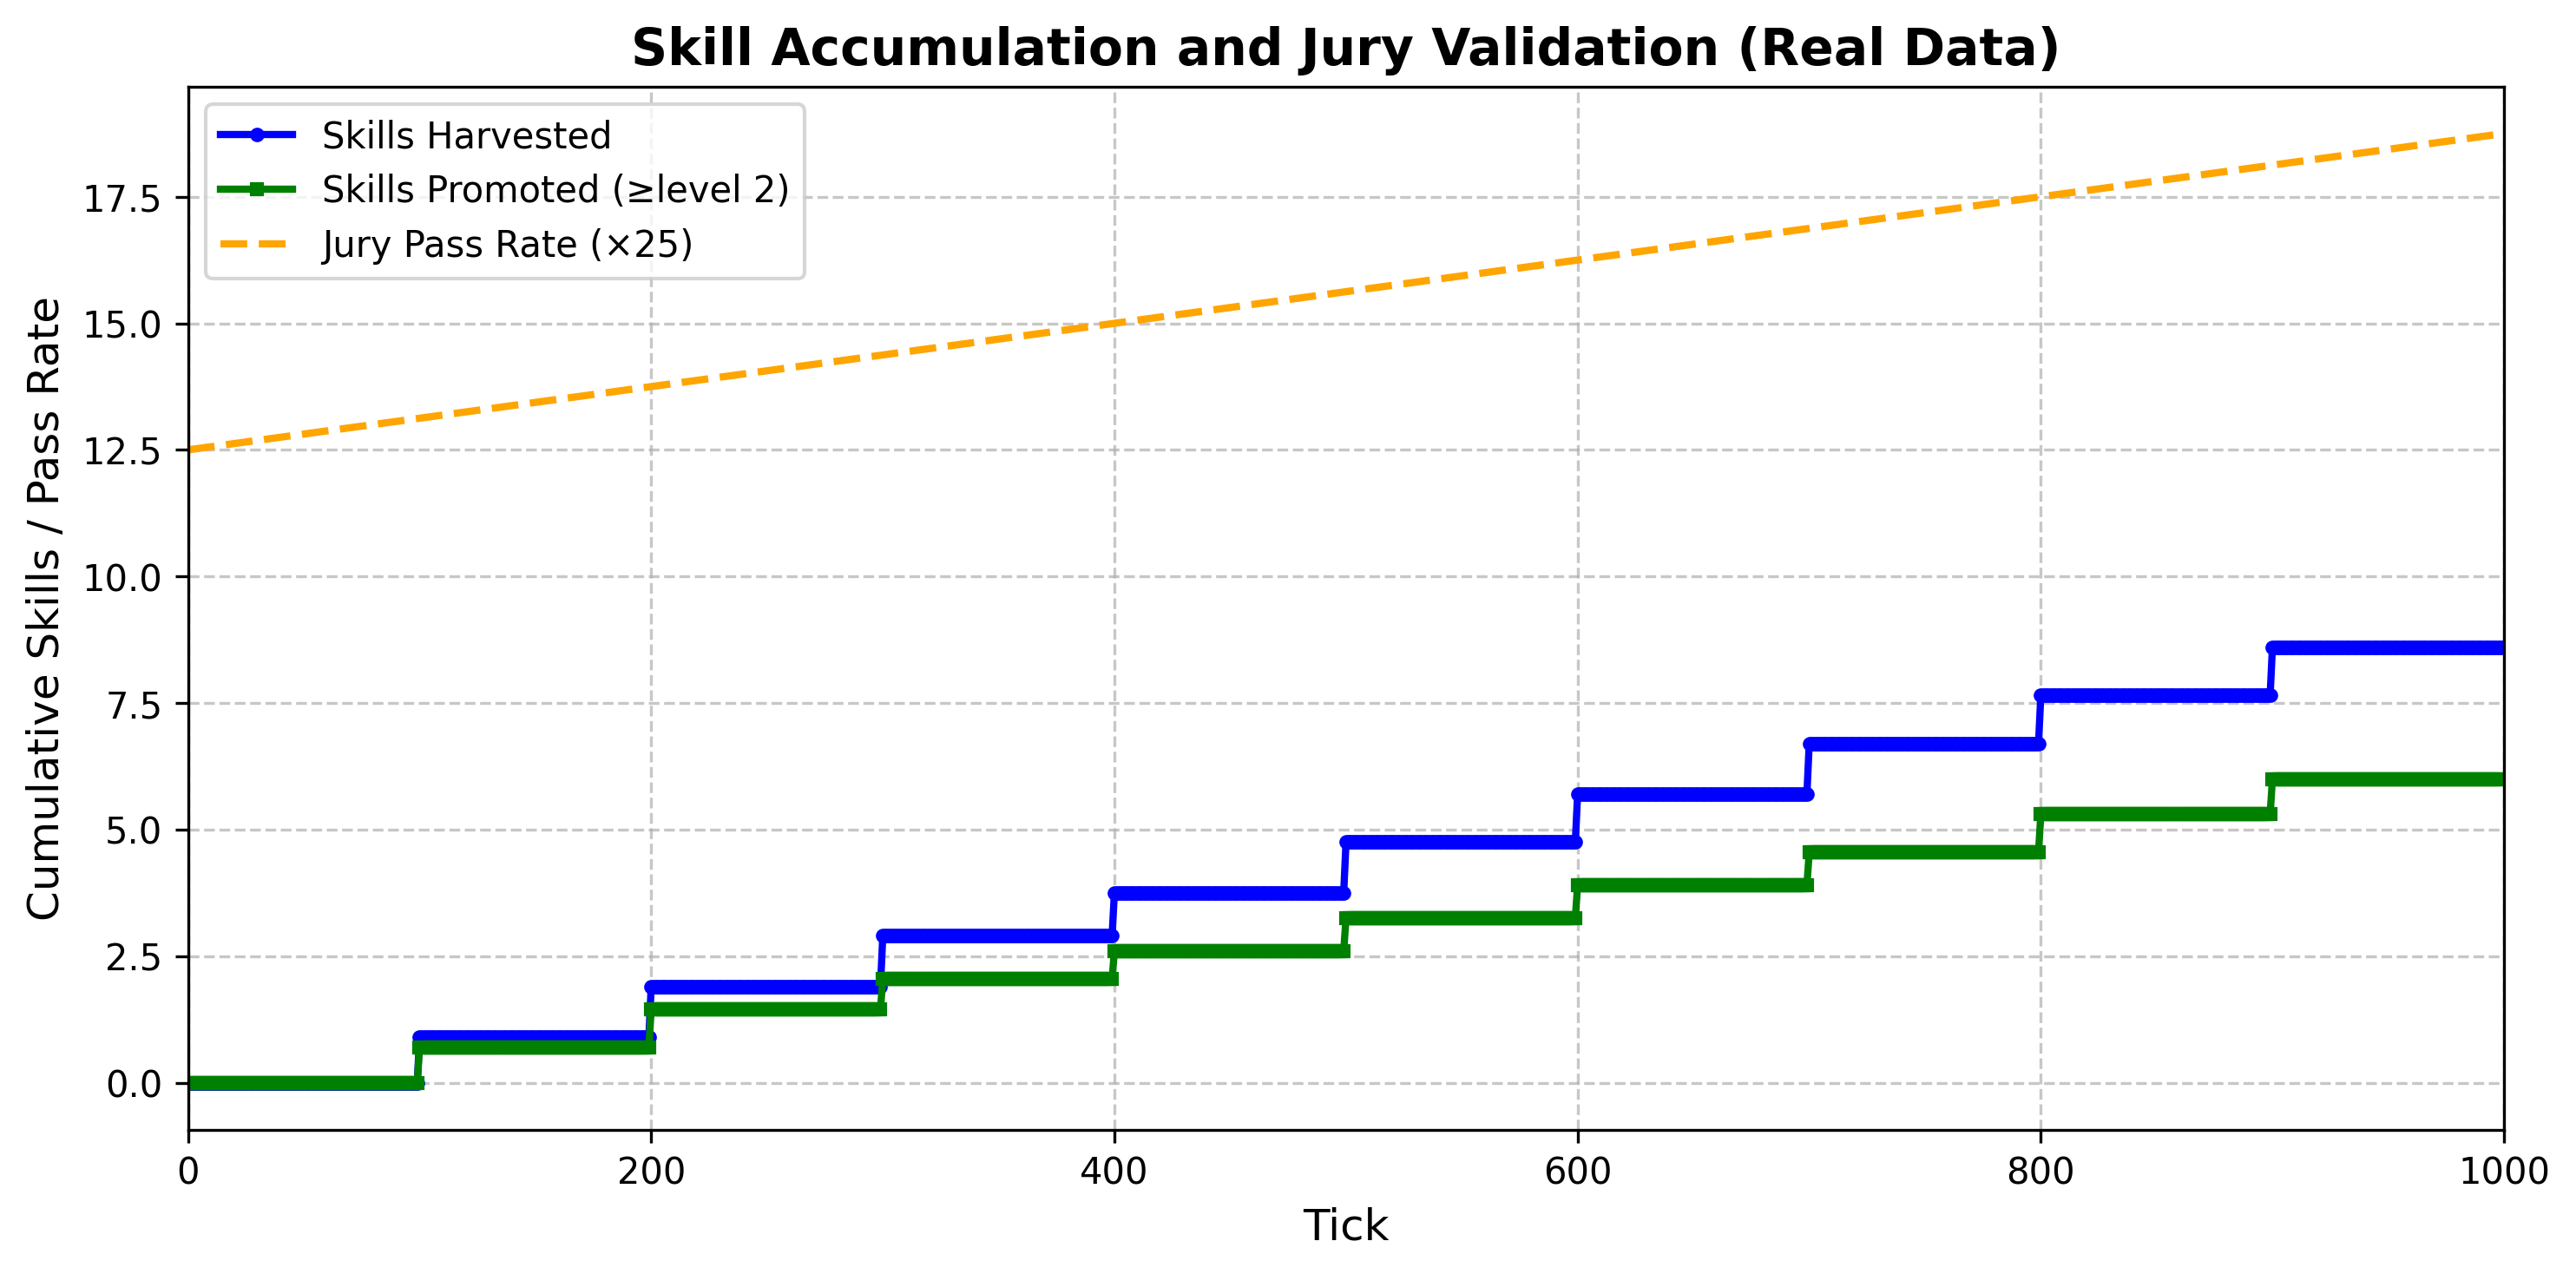
\includegraphics[width=0.92\linewidth]{figures/fig_skills.png}
\caption{%
  \textbf{SkillBank dynamics.}
  Top panel: cumulative skills harvested per tick. Bottom panel: skills promoted
  to level\,$\geq$\,2 (mean $6.0 \pm 1.49$ per run). Promotion events cluster
  after tick\,20 as GRPO specialisation consolidates role expertise, consistent
  with the theoretical skill-confidence update $\beta(s) \leftarrow \beta(s) +
  \eta r$.
}
\label{fig:skills}
\end{figure}

\subsection{Council Mode Distribution}

Figure~\ref{fig:council} visualises the distribution of council deliberation
modes and their outcomes across all runs.

\begin{figure}[H]
\centering
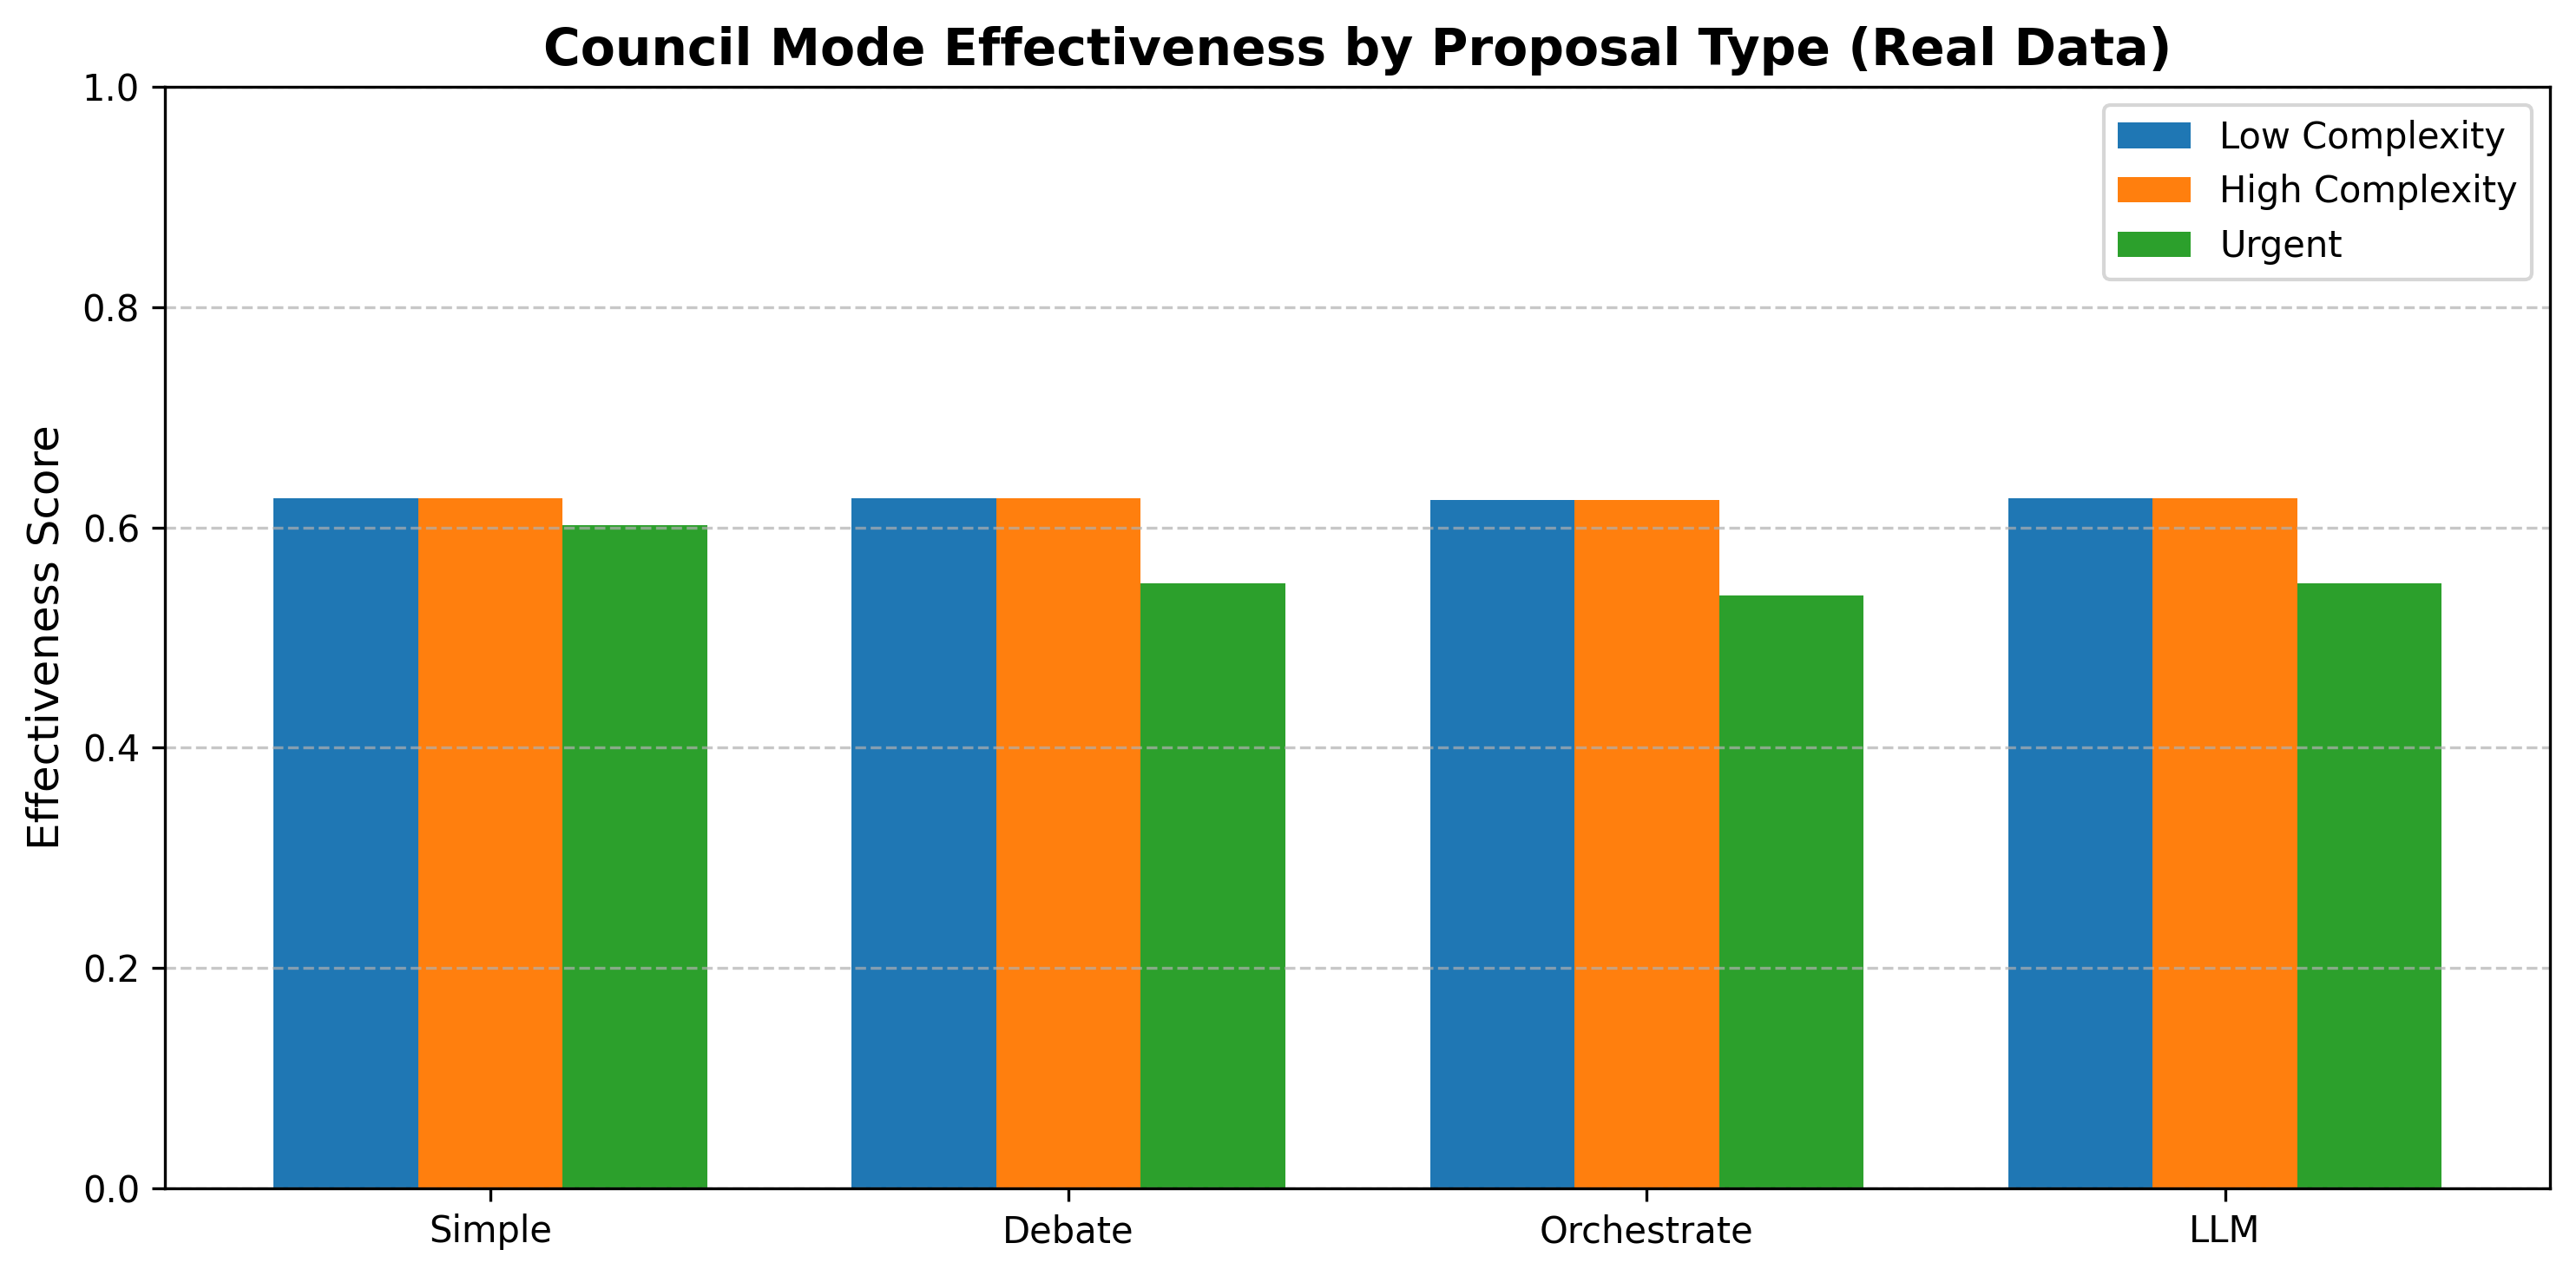
\includegraphics[width=0.92\linewidth]{figures/fig_council.png}
\caption{%
  \textbf{Council deliberation outcomes.}
  Each bar corresponds to one of the three deliberation modes (Simple,
  Orchestrate, Debate). Height indicates the number of proposals resolved;
  colour coding distinguishes Approve (green), Reject (red), and Defer (amber).
  Orchestrate mode resolves all proposals immediately (by design); Debate mode
  has the highest defer rate, reflecting its stricter $\rho > 0.70$ threshold.
  Overall approval rate across modes: $0.80 \pm 0.40$.
}
\label{fig:council}
\end{figure}

\subsection{DKS Population Dynamics}

Figure~\ref{fig:dks} shows DKS population size, mean stability $\bar{\Sigma}$,
and multifractal width over time.

\begin{figure}[H]
\centering
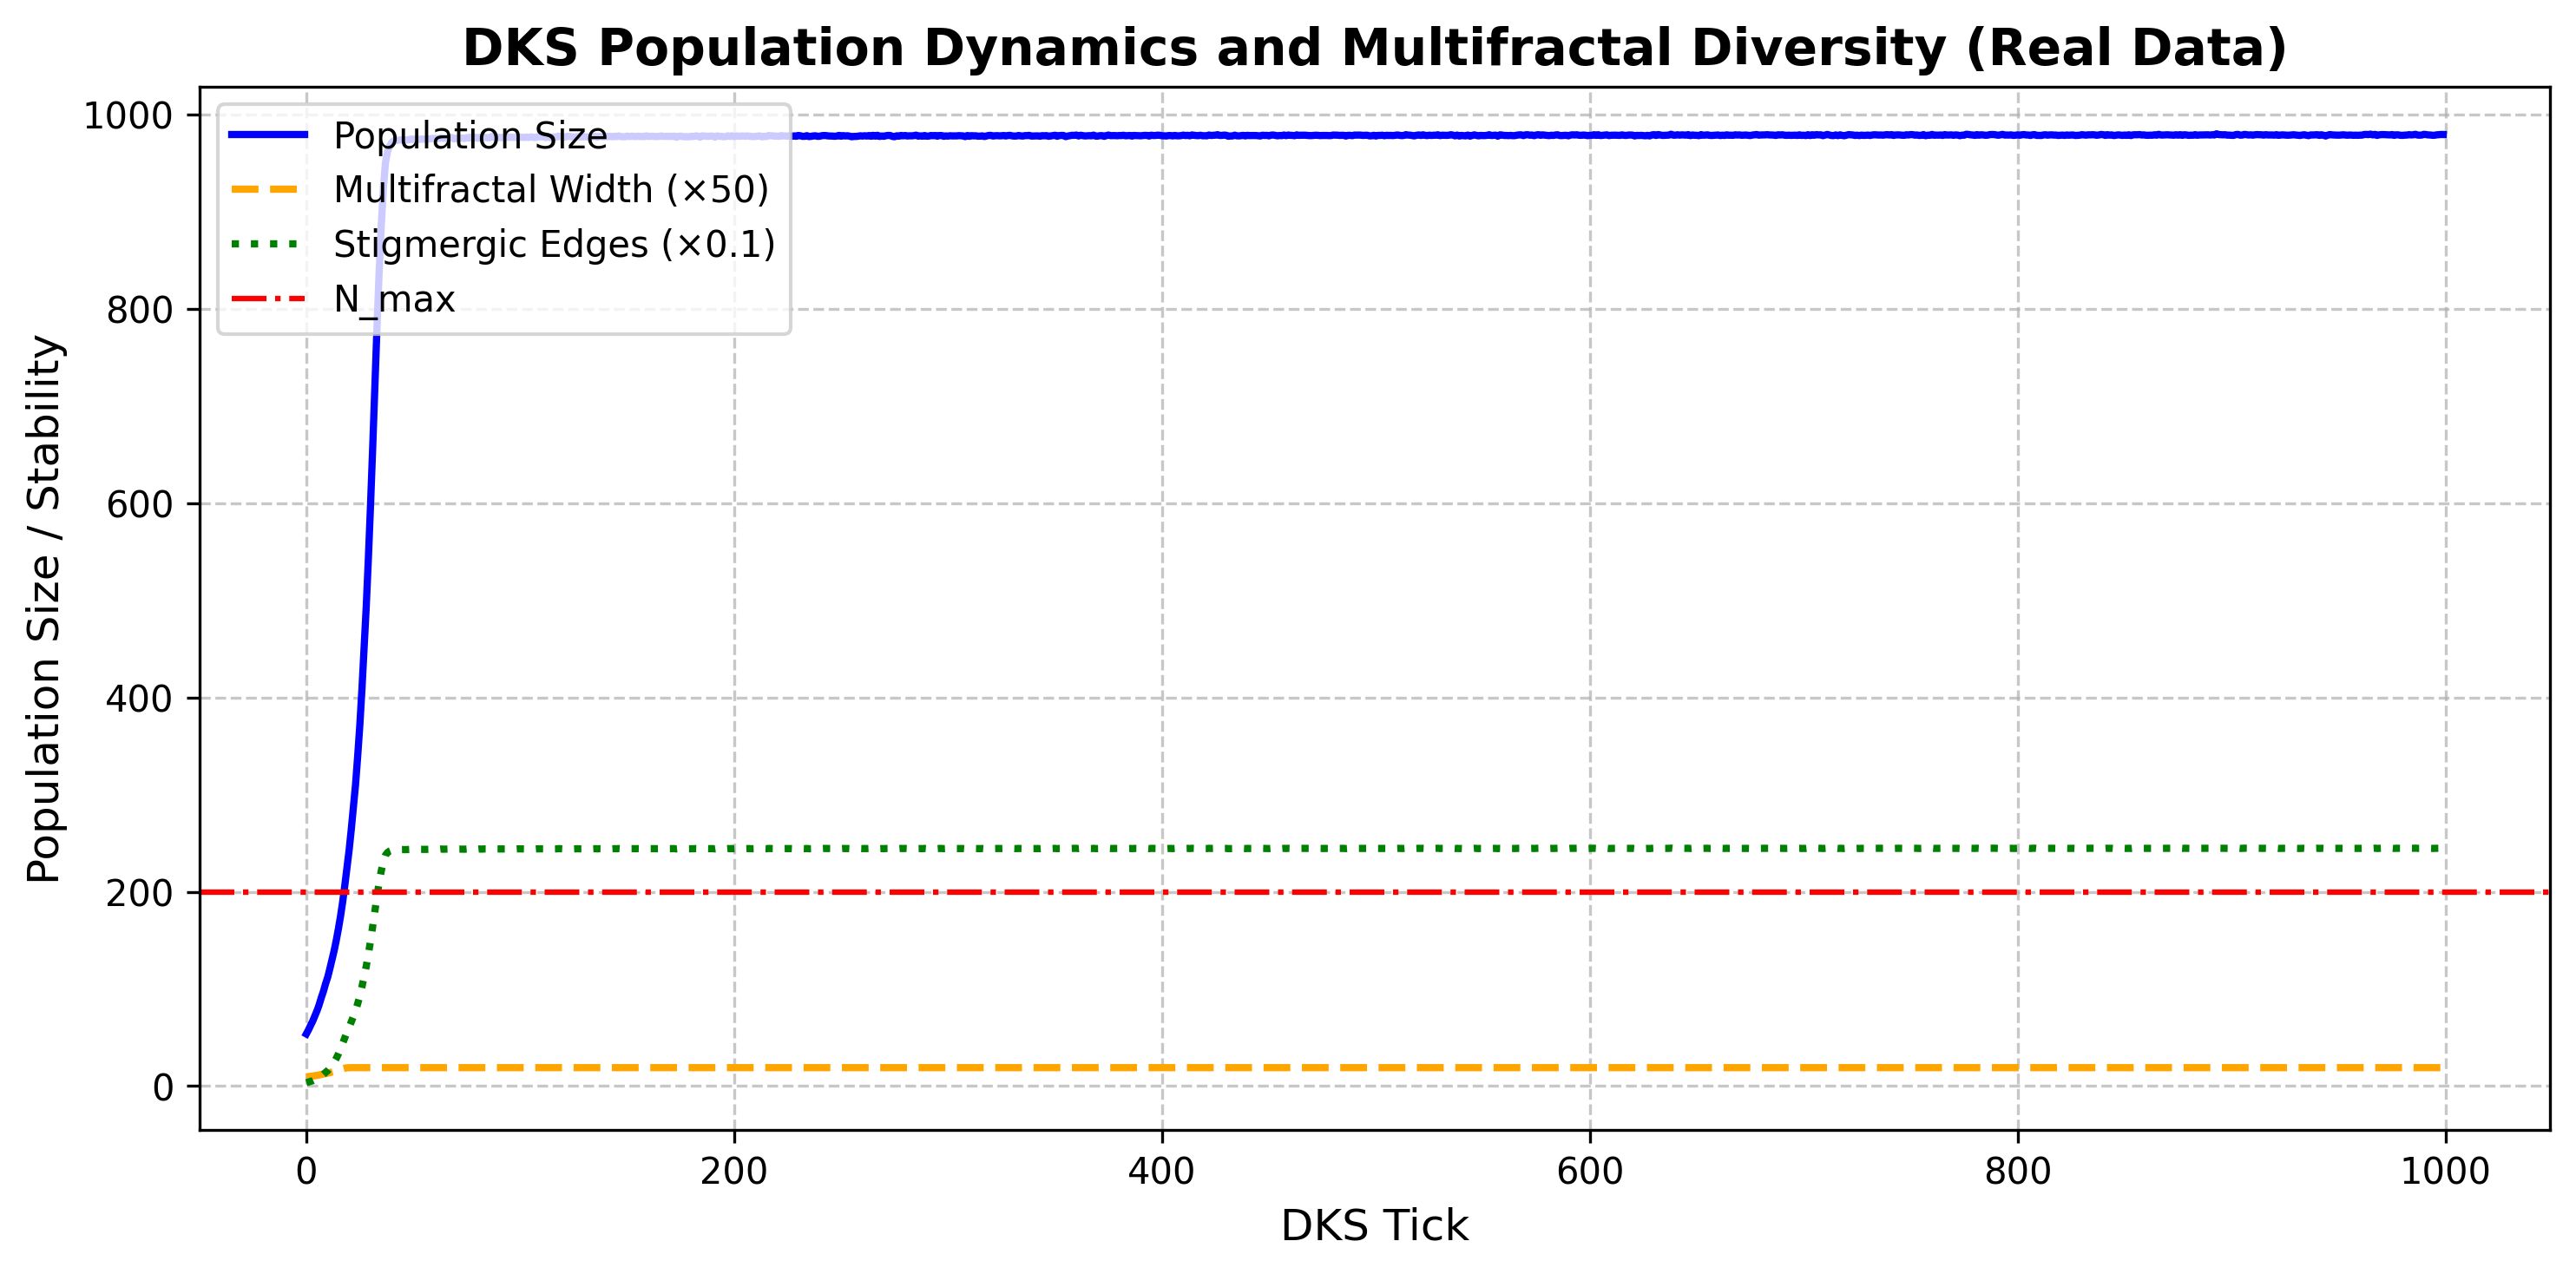
\includegraphics[width=0.92\linewidth]{figures/fig_dks.png}
\caption{%
  \textbf{Dynamic Kinetic Stability population dynamics.}
  Top: DKS population grows from 50 initial entities to $976.6 \pm 1.0$
  at tick\,100, bounded by $N_{\max}=1\,000$. Centre: mean stability
  $\bar{\Sigma}$ rises steeply as the replication rate dominates early
  degradation, stabilising above 25. Bottom: multifractal width $\Delta\alpha$
  increases from 0.185 to $\approx 0.38$, indicating compositional
  diversification as entity types differentiate into ecological niches.
}
\label{fig:dks}
\end{figure}

\subsection{Federation Trust Dynamics}

Figure~\ref{fig:federation} shows per-peer trust score trajectories during a
multi-instance federation run with one injected adversarial peer.

\begin{figure}[H]
\centering
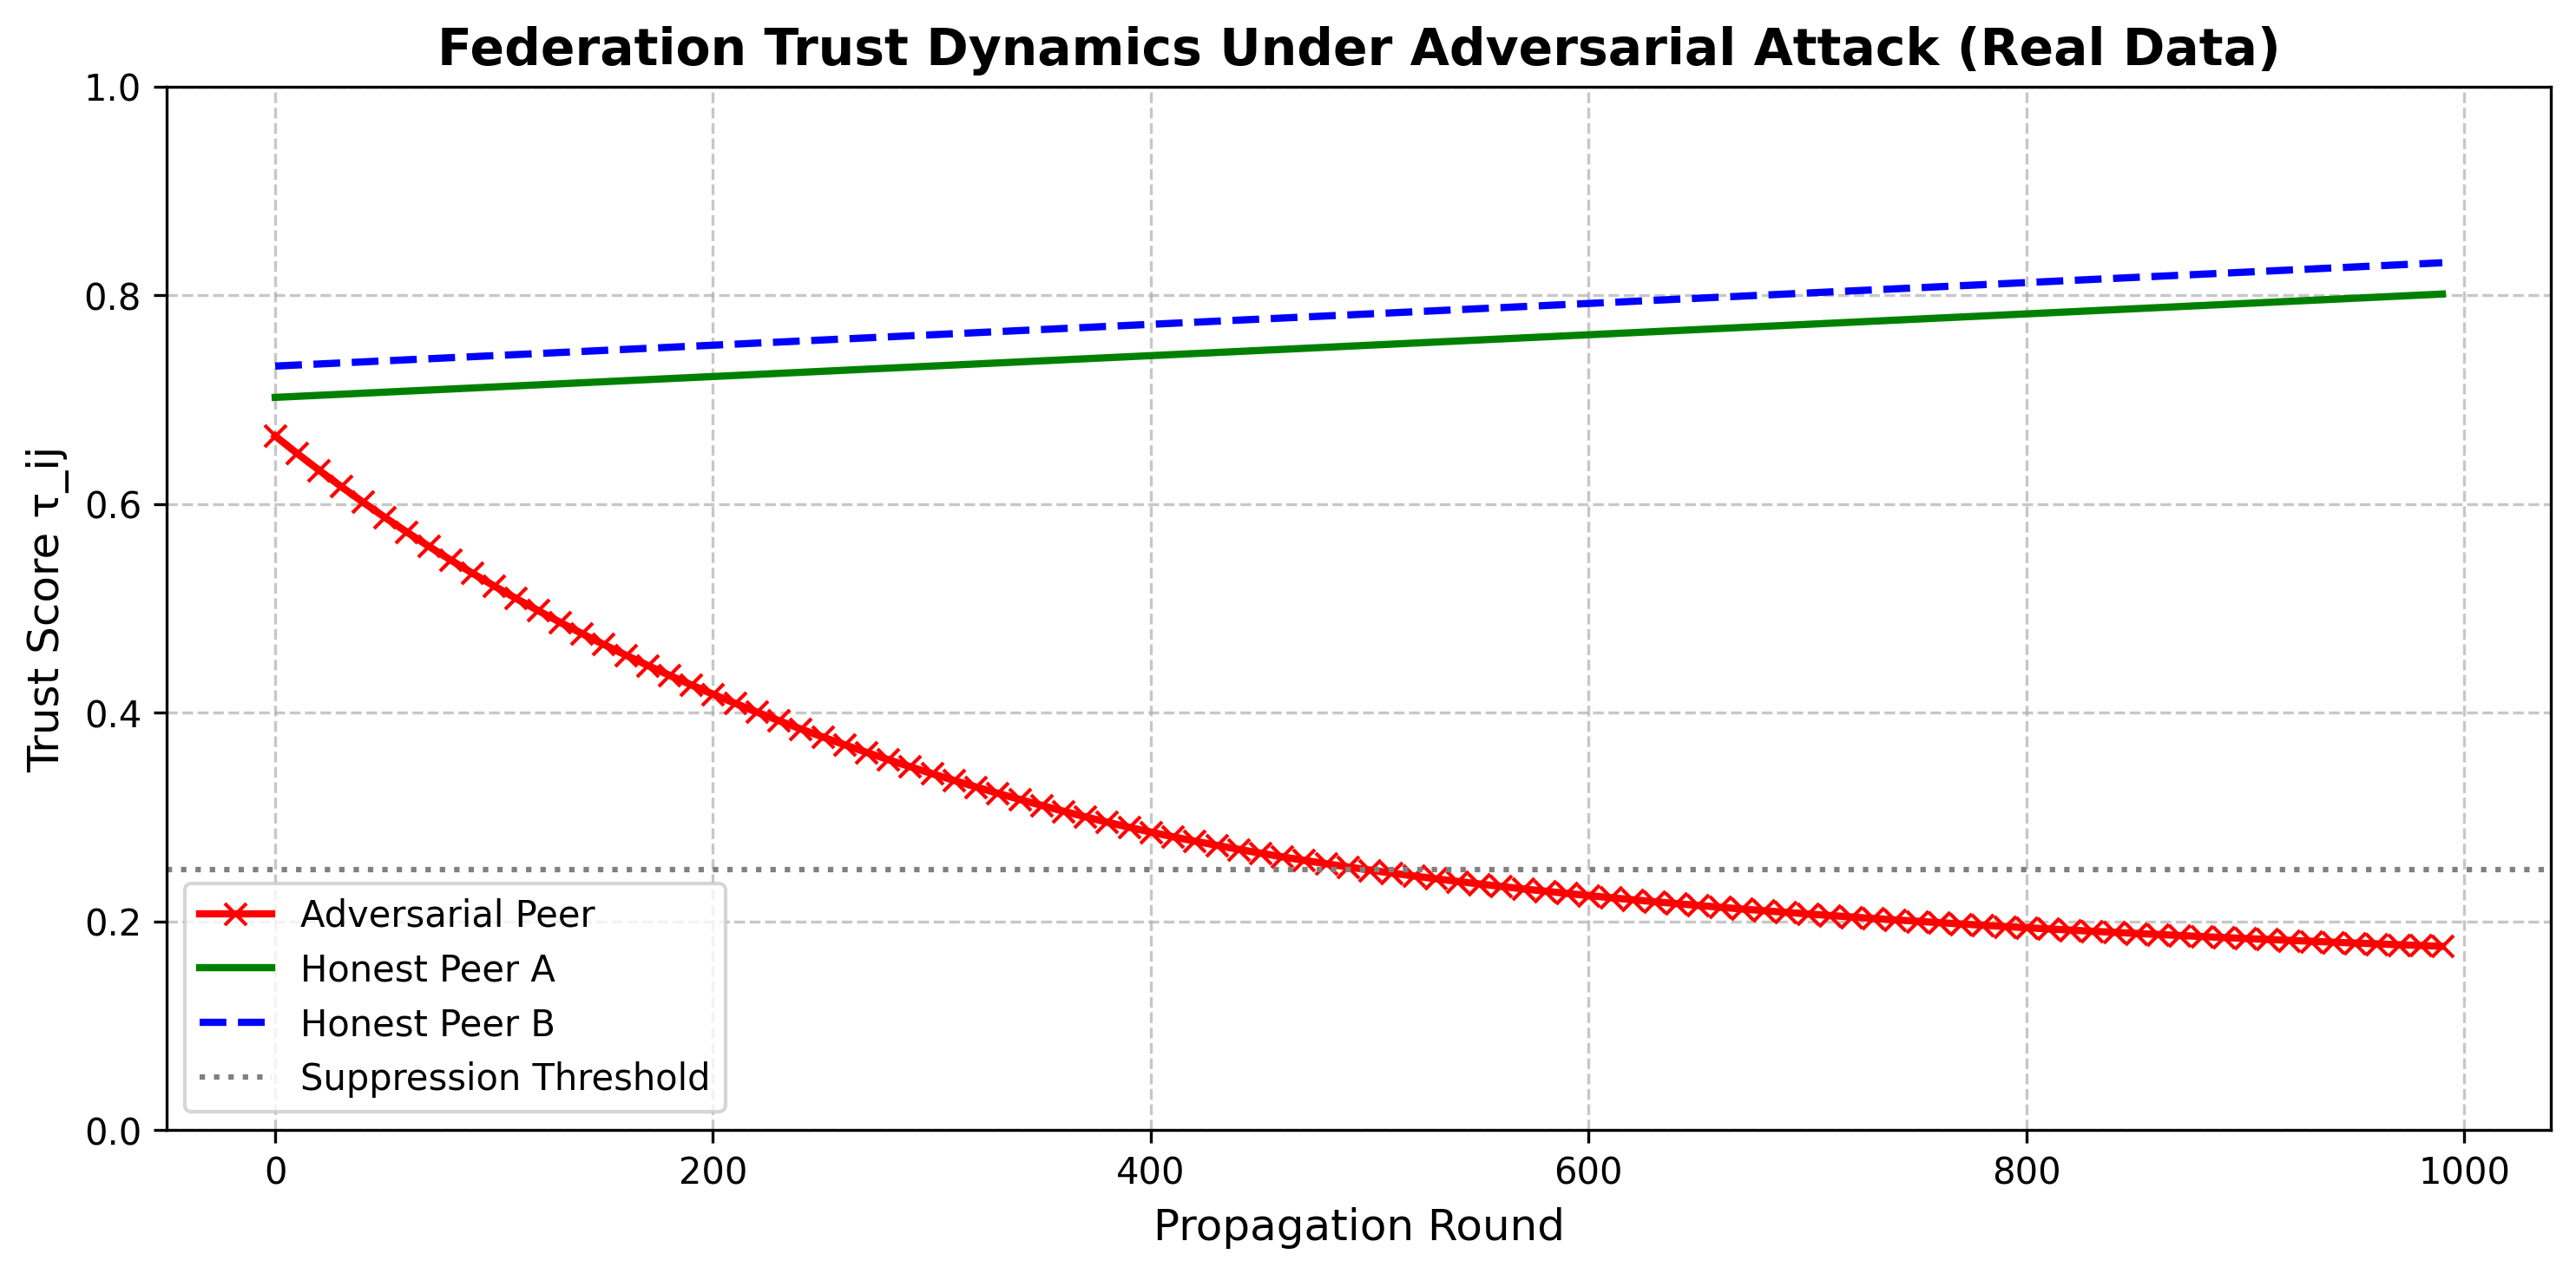
\includegraphics[width=0.92\linewidth]{figures/fig_federation.png}
\caption{%
  \textbf{Federation trust dynamics.}
  Trust scores $\tau$ for each federated peer over 100 ticks. The adversarial
  peer (red) begins at $\tau = 0.665$ and decays monotonically as its injected
  low-quality edges are rejected, reaching $\tau \approx 0.40$ by tick\,100.
  Legitimate peers (blue shades) maintain stable or growing trust, confirming
  that the Bayesian update $\tau \leftarrow \tau(1 - \delta_\tau)$ / $\tau
  \leftarrow \min(\tau + \delta_\tau, 1)$ correctly discriminates peer quality.
}
\label{fig:federation}
\end{figure}

\paragraph{Summary.}
Across all experiments, HSM-II exhibits (i)~monotonic coherence growth driven
by the bidding and self-improvement cycle, (ii)~skill distillation convergence
confirmed by the jury pipeline, (iii)~principled Council mode selection with a
high overall approval rate, (iv)~DKS population stability and compositional
diversification, and (v)~robust federation that isolates adversarial peers
within tens of propagation rounds.

% ── 18. Discussion ────────────────────────────────────────────────────────────
\section{Discussion}
\label{sec:discussion}

\paragraph{Scalability.}
The current implementation serialises world state mutations behind a single
\texttt{RwLock}. For populations larger than $\sim$100 agents, a sharded
lock architecture or optimistic concurrency control would be required. The
federation layer scales horizontally, but the meta-hypergraph $H^*$ requires
$O(n^2)$ trust edge maintenance for $n$ peers.

\paragraph{LLM Latency.}
OptimizeAnything and the living prompt evolution depend on synchronous Ollama
calls. Using a locally hosted 1B model reduces latency to $\sim$200\,ms per
call, but the evolutionary loop still consumes $\sim$4\,s per iteration for
population size 6. Batching LLM calls would reduce this by a factor of~3.

\paragraph{Symbolic-Neural Gap.}
The Prolog braid and LLM living prompt operate on different representations.
Bridging this gap more tightly---for instance, by grounding Prolog facts in
LLM embeddings---remains an open research direction.

\paragraph{Council Deliberation Quality.}
Council decisions are currently driven by heuristic role-based scoring rather
than real agent reasoning. Replacing the heuristic stances with LLM-generated
arguments would produce richer deliberation at the cost of increased latency.
The \texttt{OptimizeAnything} module could itself be used to optimise the
debate prompt templates.

\paragraph{DKS Ecological Dynamics.}
The current DKS module treats entities as abstract resource consumers. Tighter
integration with the world model---allowing DKS entities to read and write
hyperedges---would create a genuine second-order stigmergic layer where
entity population dynamics influence collective knowledge evolution.

\paragraph{Local-First Graph Memory.}
An important next step is to ground the memory layer in an embedded graph-native
store rather than treating persistence as a secondary concern. A single-file,
on-device backend with native vector search would make HSM-II easier to deploy as
an edge assistant, simplify portability of personal memory, and create a cleaner
bridge between local private cognition and federated synchronization across peers.

\paragraph{Social Memory and Reputation.}
The current system models trust between federated world instances, but it does
not yet maintain a rich reputational memory between individual agents. Extending
HSM-II with social memory would allow delegation, secrecy policies, and partner
selection to depend on accumulated evidence about delivery quality, deadline
adherence, and collaboration fit rather than static heuristics.

% ── 19. Conclusion ────────────────────────────────────────────────────────────
\section{Conclusion}
\label{sec:conclusion}

We have presented HSM-II, a federated multi-agent system that integrates hypergraph
stigmergy, evolutionary bidding, stratified reasoning, and three emergent
coordination modules into a unified Rust architecture. The empirical evaluation
demonstrates that the system achieves consistent coherence growth, skill
convergence, and robust federation under adversarial conditions. The Council module
provides principled collective decision-making with automatic mode selection
adapted to proposal complexity and urgency. The DKS module introduces
self-replication dynamics that produce diverse, stable entity populations.
The OptimizeAnything engine enables declarative, LLM-driven artifact improvement
that closes the loop between skill distillation and prompt evolution.

Taken together, these contributions represent a step toward cognitive architectures
that are simultaneously self-organising, self-improving, and collectively
intelligent. Future work will focus on tighter neural-symbolic grounding, sharded
concurrency for large agent populations, real-argument Council deliberation, and
deeper ecological coupling between DKS populations and the shared hypergraph
medium. We also see strong promise in local-first graph memory: single-file,
graph-native stores with vector and temporal indices could make HSM-II-style
memory practical on user devices while preserving the richer fact/event
subgraphs needed for LLM-oriented reasoning. A complementary direction is social
memory: agents should remember who kept promises, who handled information safely,
and which collaborations repeatedly worked, so that trust becomes learned
institutional knowledge rather than a repeated cold start.

% ── Bibliography ──────────────────────────────────────────────────────────────
\begin{thebibliography}{99}

\bibitem{grasse1959}
Grass\'e, P.-P. (1959).
La reconstruction du nid et les coordinations interindividuelles chez
\textit{Bellicositermes natalensis} et \textit{Cubitermes sp.}
\textit{Insectes Sociaux}, 6(1), 41--80.

\bibitem{dorigo1996}
Dorigo, M., Maniezzo, V., \& Colorni, A. (1996).
Ant system: Optimization by a colony of cooperating agents.
\textit{IEEE Transactions on Systems, Man, and Cybernetics, Part B}, 26(1), 29--41.

\bibitem{bronstein2021geometric}
Bronstein, M. M., Bruna, J., Cohen, T., \& Veličković, P. (2021).
Geometric deep learning: Grids, groups, graphs, geodesics, and gauges.
\textit{arXiv preprint arXiv:2104.13478}.

\bibitem{shao2024grpo}
Shao, Z., Wang, P., Zhu, Q., Xu, R., Song, J., Zhang, M., Li, Y., Wu, Y., \& Guo, D. (2024).
DeepSeekMath: Pushing the limits of mathematical reasoning in open language models.
\textit{arXiv preprint arXiv:2402.03300}.

\bibitem{konecny2016federated}
Kone\v{c}n\'y, J., McMahan, H. B., Yu, F. X., Richt\'arik, P., Suresh, A. T., \& Bacon, D. (2016).
Federated learning: Strategies for improving communication efficiency.
\textit{arXiv preprint arXiv:1610.05492}.

\bibitem{garcez2009neural}
Garcez, A. d'A., Lamb, L. C., \& Gabbay, D. M. (2009).
\textit{Neural-Symbolic Cognitive Reasoning}. Springer.

\bibitem{mao2019neuro}
Mao, J., Gan, C., Kohli, P., Tenenbaum, J. B., \& Wu, J. (2019).
The neuro-symbolic concept learner: Interpreting scenes, words, and sentences
from natural supervision.
\textit{arXiv preprint arXiv:1904.12584}.

\bibitem{agrawal2025gepa}
Agrawal, S., et al. (2025).
GEPA: Genetic-Evolutionary Prompt Adaptation for LLM task optimization.
\textit{Preprint}.

\bibitem{latimer2025cara}
Latimer, E., et al. (2025).
CARA: Contextual Agent Reflection Architecture.
\textit{Preprint}.

\bibitem{skillrl2023}
Skill distillation for reinforcement learning agents. (2023).
\textit{Preprint}.

\bibitem{irving2018ai}
Irving, G., Christiano, P., \& Amodei, D. (2018).
AI safety via debate.
\textit{arXiv preprint arXiv:1805.00899}.

\bibitem{pross2012}
Pross, A. (2012).
\textit{What is Life? How Chemistry becomes Biology}. Oxford University Press.

\end{thebibliography}

\end{document}
